%% ============================================================================
%%  Latent-Space Driven Active Learning of MLIPs for Li–LLZO Interfaces
%%  BS(Research) Thesis Presentation — Mehul Darak, IISc, April 2026
%%  Compile with: pdflatex → biber → pdflatex × 2  (or just pdflatex if no bib)
%% ============================================================================
\documentclass[aspectratio=169,10pt]{beamer}

\usepackage[T1]{fontenc}
\usepackage[utf8]{inputenc}
\usepackage{amsmath,amssymb}
\usepackage{graphicx}
\usepackage{booktabs}
\usepackage{colortbl}
\usepackage{xcolor}
\usepackage{tikz}
\usetikzlibrary{arrows.meta, positioning, shapes.geometric, fit, calc, backgrounds}
\usepackage{array}
\usepackage{multirow}
\usepackage{tcolorbox}
\tcbuselibrary{skins, breakable}
\usepackage{microtype}
\usepackage{hyperref}

\makeatletter
\setbeamertemplate{frametitle}{%
  \vskip0.08cm%
  \begin{beamercolorbox}[wd=\paperwidth,ht=0.58cm,dp=0.22cm,leftskip=0.4cm]{frametitle}%
    \usebeamerfont{frametitle}\insertframetitle%
    \ifx\insertframesubtitle\@empty\else%
      \hspace{0.6em}{\small\textcolor{iiscgold}{\insertframesubtitle}}%
    \fi%
  \end{beamercolorbox}%
  \vskip-0.04cm%
  \begin{beamercolorbox}[wd=\paperwidth,ht=0.06cm,dp=0cm]{block body}%
    \textcolor{iiscgold}{\rule{\paperwidth}{0.06cm}}%
  \end{beamercolorbox}%
}
\makeatother
%% Frametitle bar
\setbeamercolor{frametitle}{bg=iiscblue, fg=white}
\setbeamerfont{frametitle}{size=\large, series=\bfseries}
\setbeamertemplate{frametitle}{%
  \vskip0.08cm%
  \begin{beamercolorbox}[wd=\paperwidth,ht=0.58cm,dp=0.22cm,leftskip=0.4cm]{frametitle}%
    \usebeamerfont{frametitle}\insertframetitle%
    \ifx\insertframesubtitle\@empty\else%
      \hspace{0.6em}{\small\textcolor{iiscgold}{\insertframesubtitle}}%
    \fi%
  \end{beamercolorbox}%
  \vskip-0.04cm%
  \begin{beamercolorbox}[wd=\paperwidth,ht=0.06cm,dp=0cm]{block body}%
    \textcolor{iiscgold}{\rule{\paperwidth}{0.06cm}}%
  \end{beamercolorbox}%
}

%% Itemize bullets
\setbeamertemplate{itemize item}{\color{iiscblue}\small$\blacktriangleright$}
\setbeamertemplate{itemize subitem}{\color{iiscgold}$\triangleright$}
\setbeamertemplate{enumerate item}{\color{iiscblue}\textbf{\insertenumlabel.}}

%% Block colors
\setbeamercolor{block title}{bg=iiscblue, fg=white}
\setbeamercolor{block body}{bg=lightblue}
\setbeamercolor{block title alerted}{bg=badcolor, fg=white}
\setbeamercolor{block body alerted}{bg=badbg}
\setbeamercolor{block title example}{bg=wincolor, fg=white}
\setbeamercolor{block body example}{bg=winbg}

%% ── Macros ───────────────────────────────────────────────────────────────────
\newcommand{\wintext}[1]{\textcolor{wincolor}{\textbf{#1}}}
\newcommand{\badtext}[1]{\textcolor{badcolor}{\textbf{#1}}}
\newcommand{\goldtext}[1]{\textcolor{iiscgold}{\textbf{#1}}}
\newcommand{\cmark}{\textcolor{wincolor}{$\checkmark$}}
\newcommand{\xmark}{\textcolor{badcolor}{$\times$}}
\newcommand{\LLZO}{Li$_7$La$_3$Zr$_2$O$_{12}$}

%% ── Title Info ───────────────────────────────────────────────────────────────
\title[Latent-Space Driven AL for MLIPs]{%
  Latent-Space Driven Active Learning of MLIPs\\for Li--LLZO Interfaces}
\subtitle{BS(Research) Thesis Presentation}
\author[M. Darak]{%
  Mehul Darak\\[4pt]
  \small Supervisors: Prof.~Phani Motamarri \&
         Prof.~Sai Gautam Gopalakrishnan}
\institute[IISc CDS]{%
  Department of Computational and Data Sciences\\
  Indian Institute of Science, Bengaluru}
\date{April 2026}

\begin{document}

%% ============================================================================
%% SLIDE 1 — TITLE
%% ============================================================================
\begin{frame}[plain]
  \begin{tikzpicture}[remember picture, overlay]
    \fill[iiscblue]
      (current page.south west) rectangle ([yshift=1.15cm]current page.south east);
    \fill[iiscgold]
      ([yshift=1.15cm]current page.south west) rectangle
      ([yshift=1.32cm]current page.south east);
    \node[anchor=south east, xshift=-0.55cm, yshift=0.18cm]
      at (current page.south east)
      {
\includegraphics[height=0.92cm]{iisc_logo.jpg}};
    % decorative top strip
    \fill[iiscblue!15]
      (current page.north west) rectangle
      ([yshift=-0.18cm]current page.north east);
  \end{tikzpicture}
  \vspace{1.2cm}
  \titlepage
\end{frame}

%% ============================================================================
%% SLIDE 2 — MOTIVATION
%% ============================================================================
\begin{frame}{Why Does the Li\,|\,LLZO Interface Matter?}
\begin{columns}[T]
  \begin{column}{0.58\textwidth}
    \textbf{All-solid-state batteries (SSBs)} replace flammable liquid
    electrolytes with solid ionic conductors.\\[0.3em]
    \textbf{\LLZO\ (LLZO)} is among the most promising solid electrolytes:
    \begin{itemize}
      \item Ionic conductivity $\sim 10^{-3}$\,S\,cm$^{-1}$ (doped)
      \item Wide electrochemical window ($>$5\,V)
      \item Shear modulus $\sim$60\,GPa
        \hspace{0.3em}{\footnotesize(vs.~Li metal: $\sim$4.2\,GPa)}
    \end{itemize}
    \vspace{0.4em}
    \textbf{Yet the Li\,|\,LLZO interface remains the critical bottleneck:}
    \begin{itemize}
      \item ASR varies by orders of magnitude with surface preparation
      \item Dendrites penetrate despite high shear modulus
        (grain-boundary shear modulus $\sim$50\% lower than bulk)
      \item Space-charge layers alter local ionic transport
      \item Interphase evolution under cycling is termination-sensitive
    \end{itemize}
    \vspace{0.3em}
    \begin{block}{}
      \centering
      Governing failure physics of SSBs live \textbf{at the interface}.\\
      Atomic-scale understanding is both a scientific and engineering need.
    \end{block}
  \end{column}
  \begin{column}{0.4\textwidth}
    \centering
    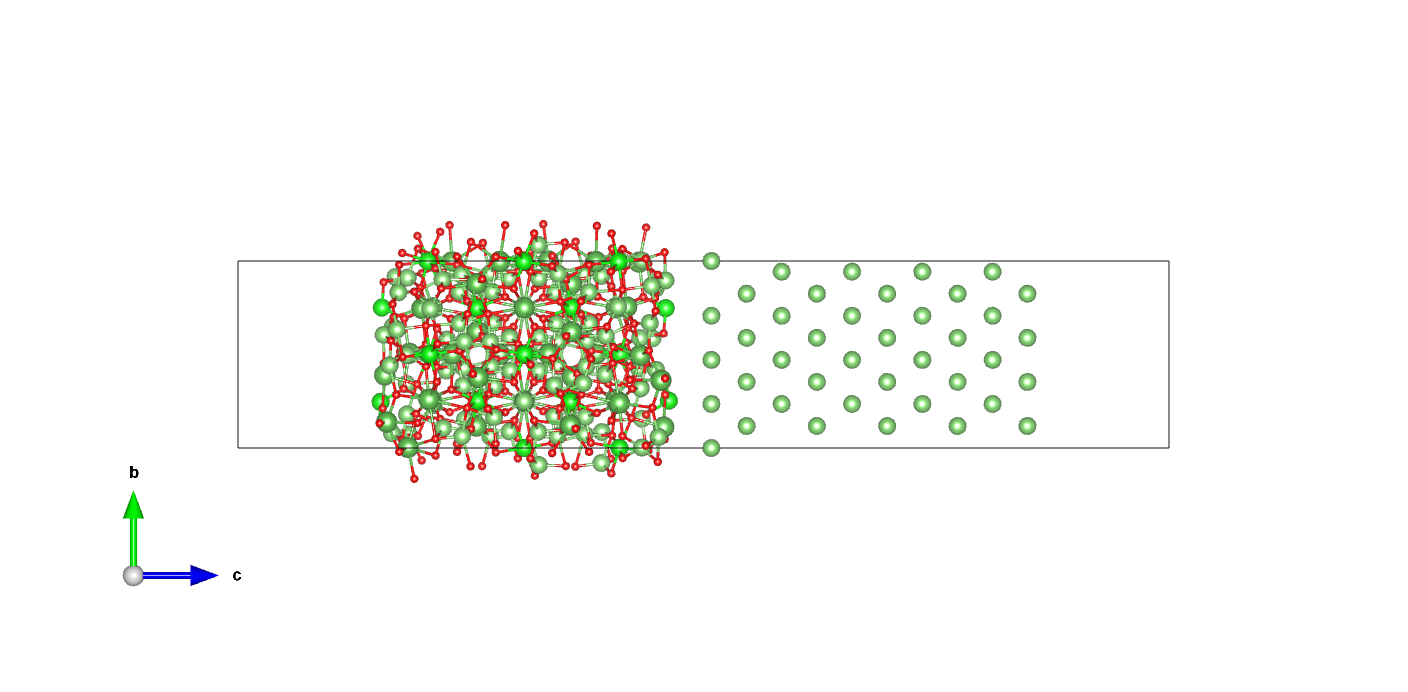
\includegraphics[width=0.88\textwidth]{Li100_LLZO_110_Zr_structure.png}\\[0.3em]
    {\footnotesize\textit{Li(100)/LLZO(110)-Zr interface model\\
    constructed in this work}}\\[0.8em]
    {\footnotesize
    \begin{tabular}{lcc}
      \toprule
      & Li metal & LLZO \\
      \midrule
      Shear mod. & 4.2 GPa & 60 GPa \\
      $\sigma_\text{ionic}$ & --- & $10^{-3}$ S/cm \\
      \bottomrule
    \end{tabular}}
  \end{column}
\end{columns}
\end{frame}

%% ============================================================================
%% SLIDE 3 — THE COMPUTATIONAL GAP
%% ============================================================================
\begin{frame}{The Computational Gap: Universal MLIPs Fail at Interfaces}
\begin{columns}[T]
  \begin{column}{0.5\textwidth}
    \textbf{DFT:} accurate, but fundamentally limited
    \begin{itemize}
      \item $<$500 atoms, $<$50 ps
      \item Interface supercells: 500--1500 atoms \xmark
      \item Li-site disorder: $>$65,000 configurations \xmark
      \item Non-periodic BCs require workarounds \xmark
    \end{itemize}

    \vspace{0.5em}
    \textbf{Universal MLIPs} (MACE-MP, MACE-OMAT):\\
    Pretrained on millions of bulk/slab configurations
    \begin{itemize}
      \item Broad chemical coverage \cmark
      \item Fast inference \cmark
      \item \badtext{Systematic PES softening} at surfaces,
        defects, interfaces \textit{[Deng et al., 2025]} \xmark
      \item Interface atoms are \badtext{out-of-distribution} \xmark
    \end{itemize}
  \end{column}
  \begin{column}{0.48\textwidth}
    \begin{alertblock}{Universal MACE-OMAT on Li--LLZO Interfaces}
      \centering\vspace{0.2em}
      \begin{tabular}{lc}
        \toprule
        Metric & Value \\
        \midrule
        Energy RMSE & \badtext{606 meV/atom} \\
        Force RMSE  & \badtext{136 meV/\AA} \\
        \bottomrule
      \end{tabular}\vspace{0.2em}
    \end{alertblock}

    \vspace{0.5em}
    \begin{exampleblock}{After targeted fine-tuning (this work)}
      \centering\vspace{0.2em}
      \begin{tabular}{lc}
        \toprule
        Metric & Value \\
        \midrule
        Energy RMSE & \wintext{$<$5 meV/atom} \\
        Force RMSE  & \wintext{$\sim$50 meV/\AA} \\
        \bottomrule
      \end{tabular}\vspace{0.2em}
    \end{exampleblock}

    \vspace{0.6em}
    \centering
    \textbf{With only \goldtext{26 DFT-labeled structures}.}\\[0.3em]
    \textit{How? By choosing them optimally using latent space.}
  \end{column}
\end{columns}
\end{frame}

%% ============================================================================
%% SLIDE 4 — FRAMEWORK OVERVIEW
%% ============================================================================
\begin{frame}{Our Framework: Latent-Space Driven Active Learning}
\begin{center}
\resizebox{0.98\textwidth}{!}{%
\begin{tikzpicture}[
  node distance=0.55cm and 0.75cm,
  box/.style={rectangle, rounded corners=5pt, draw=iiscblue, very thick,
              fill=lightblue, text centered,
              minimum height=1.0cm, minimum width=2.4cm, font=\bfseries\small},
  sbox/.style={rectangle, rounded corners=5pt, draw=iiscgold, very thick,
               fill=lightgold, text centered,
               minimum height=1.0cm, minimum width=2.4cm, font=\bfseries\small},
  arr/.style={-{Stealth[scale=1.4]}, very thick, iiscblue},
  looparr/.style={-{Stealth[scale=1.4]}, thick, dashed, iiscgold},
  lbl/.style={font=\scriptsize, text=neutgray, text centered},
]
  \node[box] (slabs) {Interface\\Construction};
  \node[box, right=of slabs] (md)  {MD Sampling\\(NVT)};
  \node[box, right=of md]    (emb) {Latent Space\\Extraction};
  \node[sbox, right=of emb]  (fps) {FPS / Super-FPS};
  \node[box, right=of fps]   (dft) {DFT-FE\\Labeling};
  \node[sbox, below=0.85cm of fps] (lora) {LoRA\\Fine-Tuning};

  \draw[arr] (slabs) -- (md);
  \draw[arr] (md)    -- (emb);
  \draw[arr] (emb)   -- (fps);
  \draw[arr] (fps)   -- (dft);
  \draw[arr] (dft)   |- (lora);
  \draw[looparr] (lora.west) -- +(-0.6,0) |- (md.south);

  \node[lbl, below=0.18cm of slabs] {3 Li orient.\\6 LLZO terms.};
  \node[lbl, below=0.18cm of md]    {550K \& 1100K\\$\sim$5000 frames};
  \node[lbl, below=0.18cm of emb]   {256-dim\\mean-pooled};
  \node[lbl, above=0.18cm of fps]   {\textcolor{iiscgold}{\bfseries Novel}};
  \node[lbl, below=0.18cm of dft]   {Frontier HPC\\450--1500 atoms};
  \node[lbl, right=0.2cm of lora]   {rank-5 LoRA\\$<$1\% params};

  \begin{scope}[on background layer]
    \node[draw=iiscgold, dashed, very thick, rounded corners=8pt,
          fill=iiscgold!5,
          fit=(md)(emb)(fps)(dft)(lora), inner sep=6pt,
          label={[iiscgold, font=\small\bfseries]above:Active Learning Loop}] {};
  \end{scope}
\end{tikzpicture}}
\end{center}
\vspace{0.15em}
\begin{columns}
  \begin{column}{0.5\textwidth}
    \textbf{Key design choices:}
    \begin{itemize}
      \item Latent space $\gg$ hand-crafted descriptors for diversity
      \item LoRA preserves pretrained general chemistry
    \end{itemize}
  \end{column}
  \begin{column}{0.5\textwidth}
    \textbf{Two complete iterations:}
    \begin{itemize}
      \item \textbf{26 total DFT calculations}
      \item Energy RMSE: $607 \to 4.7$\,meV/atom
      \item Validated on OOD, energetics, and MD
    \end{itemize}
  \end{column}
\end{columns}
\end{frame}

%% ============================================================================
%% SLIDE 5 — INTERFACE CONSTRUCTION
%% ============================================================================
\begin{frame}{Step 1: Constructing a Diverse Interface Pool}
\begin{columns}[T]
  \begin{column}{0.53\textwidth}
    \textbf{Li slabs:} BCC, $a = 3.51$\,\AA\ — orientations (100), (110), (111)\\[0.4em]
    \textbf{LLZO slabs:} DFT-optimized surfaces from
    \textbf{Canepa, Dawson, Sai Gautam et al.\ (2018)}:
    \begin{itemize}
      \item Zr-terminated: (001), (110)
      \item La-terminated: (010), (011)
      \item Li-terminated: (021), (110)
    \end{itemize}
    \vspace{0.4em}
    \textbf{Lattice matching:} $(m\!\times\!n)$ supercell search,
    anisotropic scaling of Li to match LLZO in-plane.\\
    Criterion: mismatch $<10\%$ in both directions.\\[0.3em]
    \textbf{Gap optimization:} MACE-OMAT energy scan
    $d \in \{1.0, 1.5, \ldots, 4.0\}$\,\AA; optimal gap $\approx 2$--3\,\AA\\[0.3em]
    \textbf{Relaxation:} FIRE algorithm until $F_\text{max} < 0.05$\,eV/\AA\\[0.3em]
    \begin{block}{Outcome}
      18 candidate interfaces constructed;
      \textbf{13 converge} after relaxation.\\
      System sizes: 450--1500 atoms.
    \end{block}
  \end{column}
  \begin{column}{0.45\textwidth}
    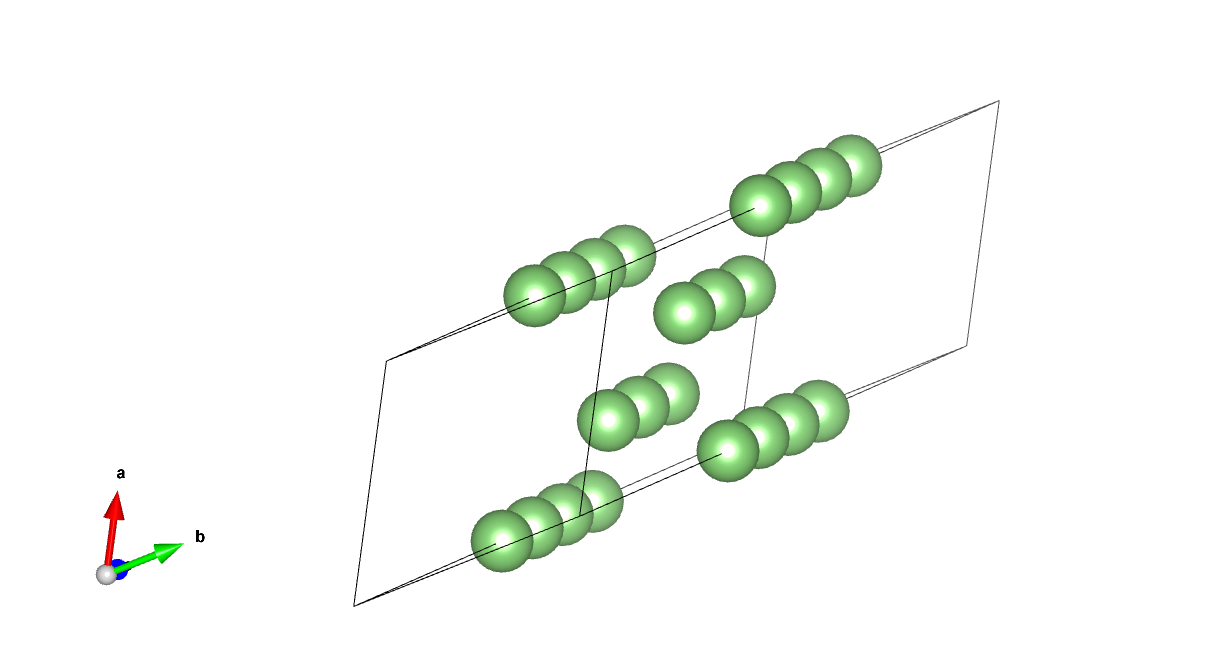
\includegraphics[width=0.49\textwidth]{Li111_pre_mismatch.png}
    \hfill
    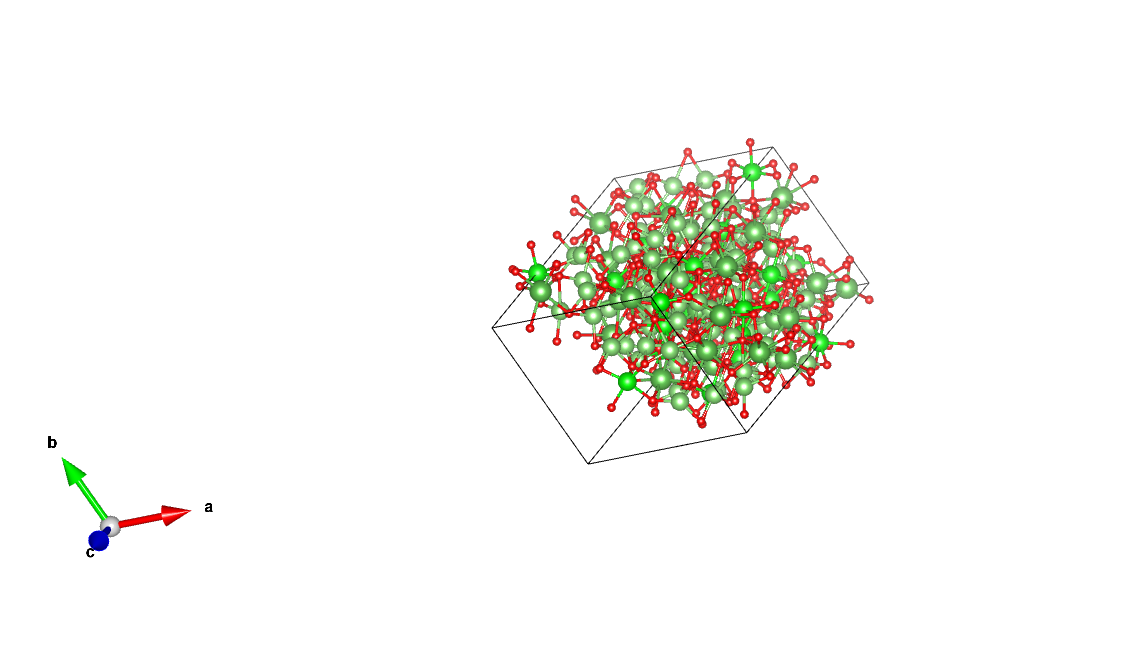
\includegraphics[width=0.49\textwidth]{LLZO_mismatch_example.png}\\[0.15em]
    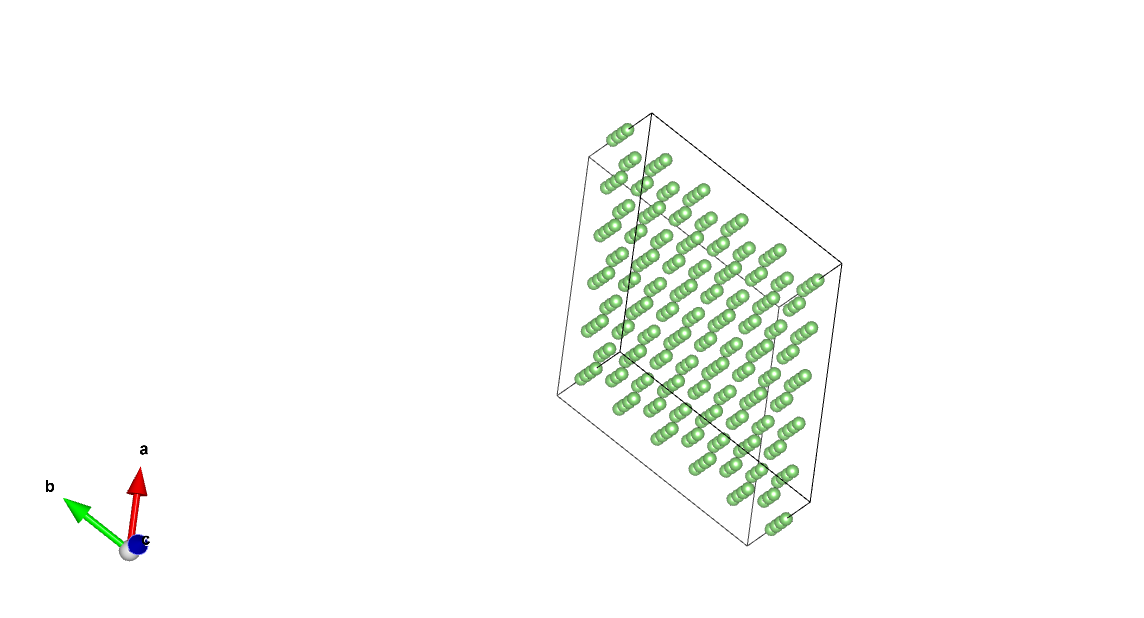
\includegraphics[width=0.49\textwidth]{Li111_after_mismatchScript.png}
    \hfill
    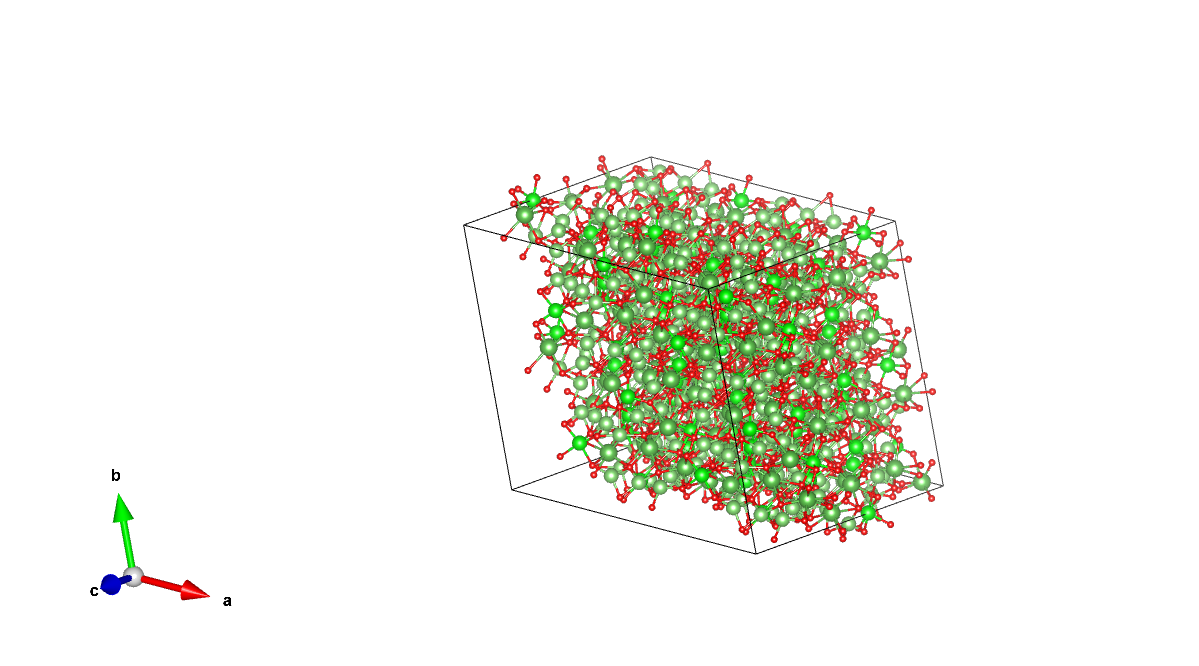
\includegraphics[width=0.49\textwidth]{LLZO_110_aftermatch.png}\\[0.2em]
    {\footnotesize\textit{Top: pre-match. Bottom: post-match.\\
    Li(111)\,|\,LLZO(110) example: $a_\text{Li} = 4.96$\,\AA\ $\to$
    matched to LLZO $a = 22.59$\,\AA.}}
  \end{column}
\end{columns}
\end{frame}

%% ============================================================================
%% SLIDE 6 — LATENT SPACE + FPS CONCEPT
%% ============================================================================
\begin{frame}{Step 2: Guiding Selection with the Model's Own Latent Space}
\begin{columns}[T]
  \begin{column}{0.5\textwidth}
    \textbf{MACE latent embeddings:}
    \begin{itemize}
      \item Per-atom: $\ell\!=\!0$ (rotationally invariant) components of final
        message-passing layer, $\mathbf{z}_i \in \mathbb{R}^{256}$
      \item Structure-level: mean pooling
        $\mathbf{Z}_S = \frac{1}{N_S}\sum_i \mathbf{z}_i$
      \item Encodes \textit{learned} many-body chemical similarity\\
        — stronger signal than SOAP or CUR on geometric descriptors
    \end{itemize}

    \vspace{0.5em}
    \textbf{Farthest Point Sampling (FPS):}
    \begin{equation*}
      k^* = \operatorname*{arg\,max}_{k \in \mathcal{P}}\;
            \min_{s \in \mathcal{S}} \|\mathbf{Z}_k - \mathbf{Z}_s\|_2
    \end{equation*}
    Greedy $k$-center. No ensemble required.\\[0.3em]
    \textbf{Why not uncertainty sampling?}\\
    UQ (QBC, deep ensembles) fails under distribution shift — exactly the interface OOD scenario. FPS directly maximizes coverage of unexplored chemical space.
  \end{column}
  \begin{column}{0.48\textwidth}
    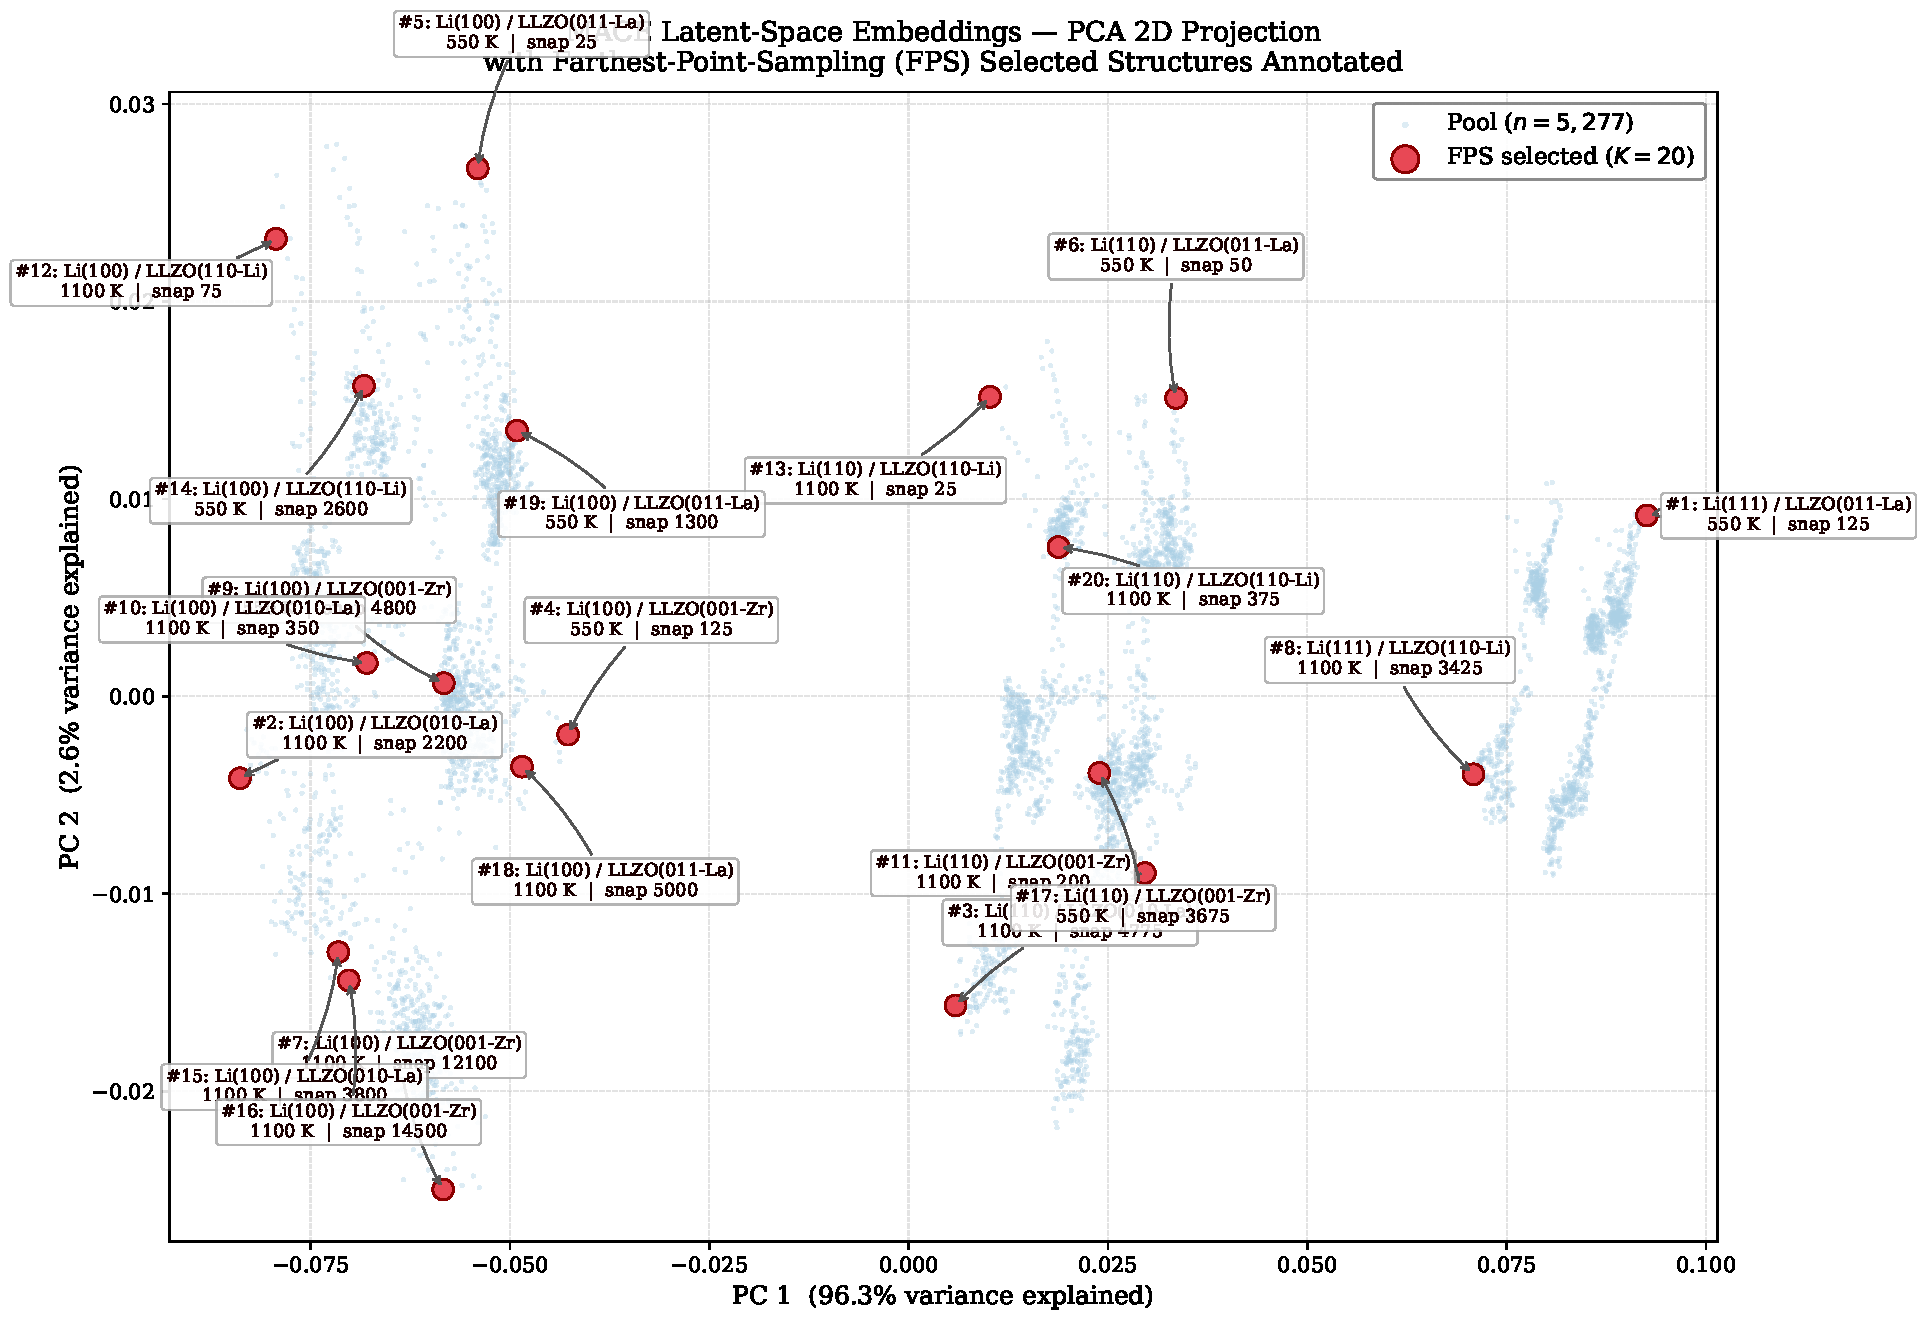
\includegraphics[width=\textwidth]{fps_embedding_2d.pdf}
    {\footnotesize\textit{2D PCA of 5,297-structure pool (PC1 vs PC2). Red: 20 FPS-selected structures, annotated by interface type and MD temperature. FPS was done in 32D; proximity in 2D does not imply redundancy.}}
  \end{column}
\end{columns}
\end{frame}

%% ============================================================================
%% SLIDE 7 — FPS COVERAGE STATS (ITERATION 0)
%% ============================================================================
\begin{frame}{Iteration 0: Coverage Statistics Validate Selection Quality}
\begin{columns}[T]
  \begin{column}{0.45\textwidth}
    \textbf{Pool:} 5,297 structures (filtered by $E > 0$)\\
    \textbf{Selected:} $K\!=\!20$ via FPS in 32-dim PCA space
    \hspace{0.3em}($\geq 99.9\%$ variance retained)\\[0.4em]

    \begin{tabular}{lc}
      \toprule
      Coverage metric & Value \\
      \midrule
      Mean $\bar{\delta}_k$              & 0.0093 \\
      Median $\delta_{50}$               & 0.0097 \\
      95\textsuperscript{th} pctile      & 0.0148 \\
      Coverage radius $\rho$             & 0.0176 \\
      Min pairwise distance              & 0.0180 \\
      \bottomrule
    \end{tabular}

    \vspace{0.5em}
    Three consistency checks:
    \begin{itemize}
      \item Min pairwise dist $>$ $\rho$
        $\Rightarrow$ \wintext{zero redundancy}
      \item PCA distortion: mean 0.02\%
        $\Rightarrow$ \wintext{geometric fidelity}
      \item Centering/vacuum change: $\Delta\ell_2 = 1.2\!\times\!10^{-6}$
        $\Rightarrow$ \wintext{embeddings encode chemistry, not geometry}
    \end{itemize}
    \vspace{0.3em}
    FPS preference for 1100\,K structures (60\%): larger phase-space excursions
    $\Rightarrow$ boundary of latent manifold \wintext{exactly what AL needs}.
  \end{column}
  \begin{column}{0.53\textwidth}
    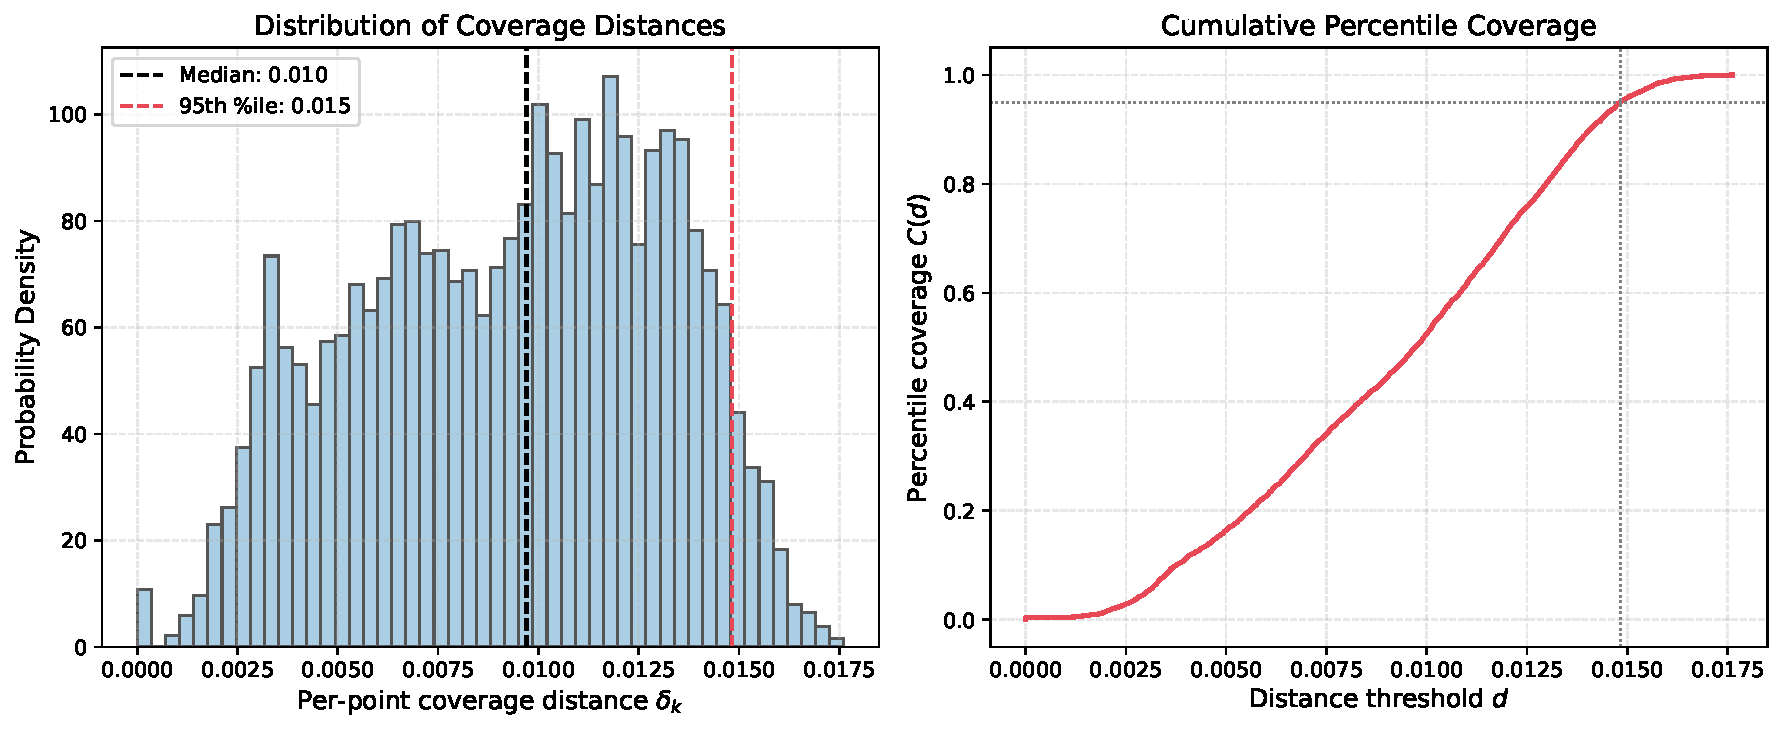
\includegraphics[width=\textwidth]{coverage_statistics.pdf}\\[0.2em]
    {\footnotesize\textit{(a) Per-point coverage distance $\delta_k$ PDF.
    (b) Cumulative coverage $C(d)$: 95\% of pool is within $d\!=\!0.0148$
    of a selected structure.}}
  \end{column}
\end{columns}
\end{frame}

%% ============================================================================
%% SLIDE 8 — SUPER-FPS (NOVEL CONTRIBUTION)
%% ============================================================================
\begin{frame}{Super-FPS: Novel Two-Stage Selection for Large Pools}
                                                              \framesubtitle{(Novel contribution of this work)}
\begin{columns}[T]
  \begin{column}{0.5\textwidth}
    \textbf{Problem in Iteration 1:} $\sim$1,320 pool structures including external geometries.
    We want only $K\!=\!6$ DFT calls.
    Naïve FPS seeded with full $\mathcal{T}$ is brittle at this scale.\\[0.5em]

    \textbf{Two-stage Super-FPS:}
    \begin{enumerate}
      \item \textbf{Coarse pass} — FPS seeded with random
        subset $\mathcal{R} \!\subset\! \mathcal{T}$,
        selects $M\!=\!20$ candidates $\mathcal{Q}$:\\
        $\mathcal{Q} = \mathrm{FPS}(\mathcal{P},\,\mathcal{R},\,20)$
      \item \textbf{Fine pass} — FPS seeded with \textit{full}
        training set $\mathcal{T}$, selects $K\!=\!6$ structures:\\
        $\mathcal{L} = \mathrm{FPS}(\mathcal{Q},\,\mathcal{T},\,6)$
    \end{enumerate}

    \vspace{0.4em}
    \begin{block}{Coverage result}
      6 structures $\Rightarrow$ nearest-neighbor for \textbf{922/1320 pool points (69.8\%)}.\\
      2 external structures lie \textbf{$1.5$--$2\times$ beyond MD pool $\rho$} — unreachable by any MD trajectory.
    \end{block}
  \end{column}
  \begin{column}{0.48\textwidth}
    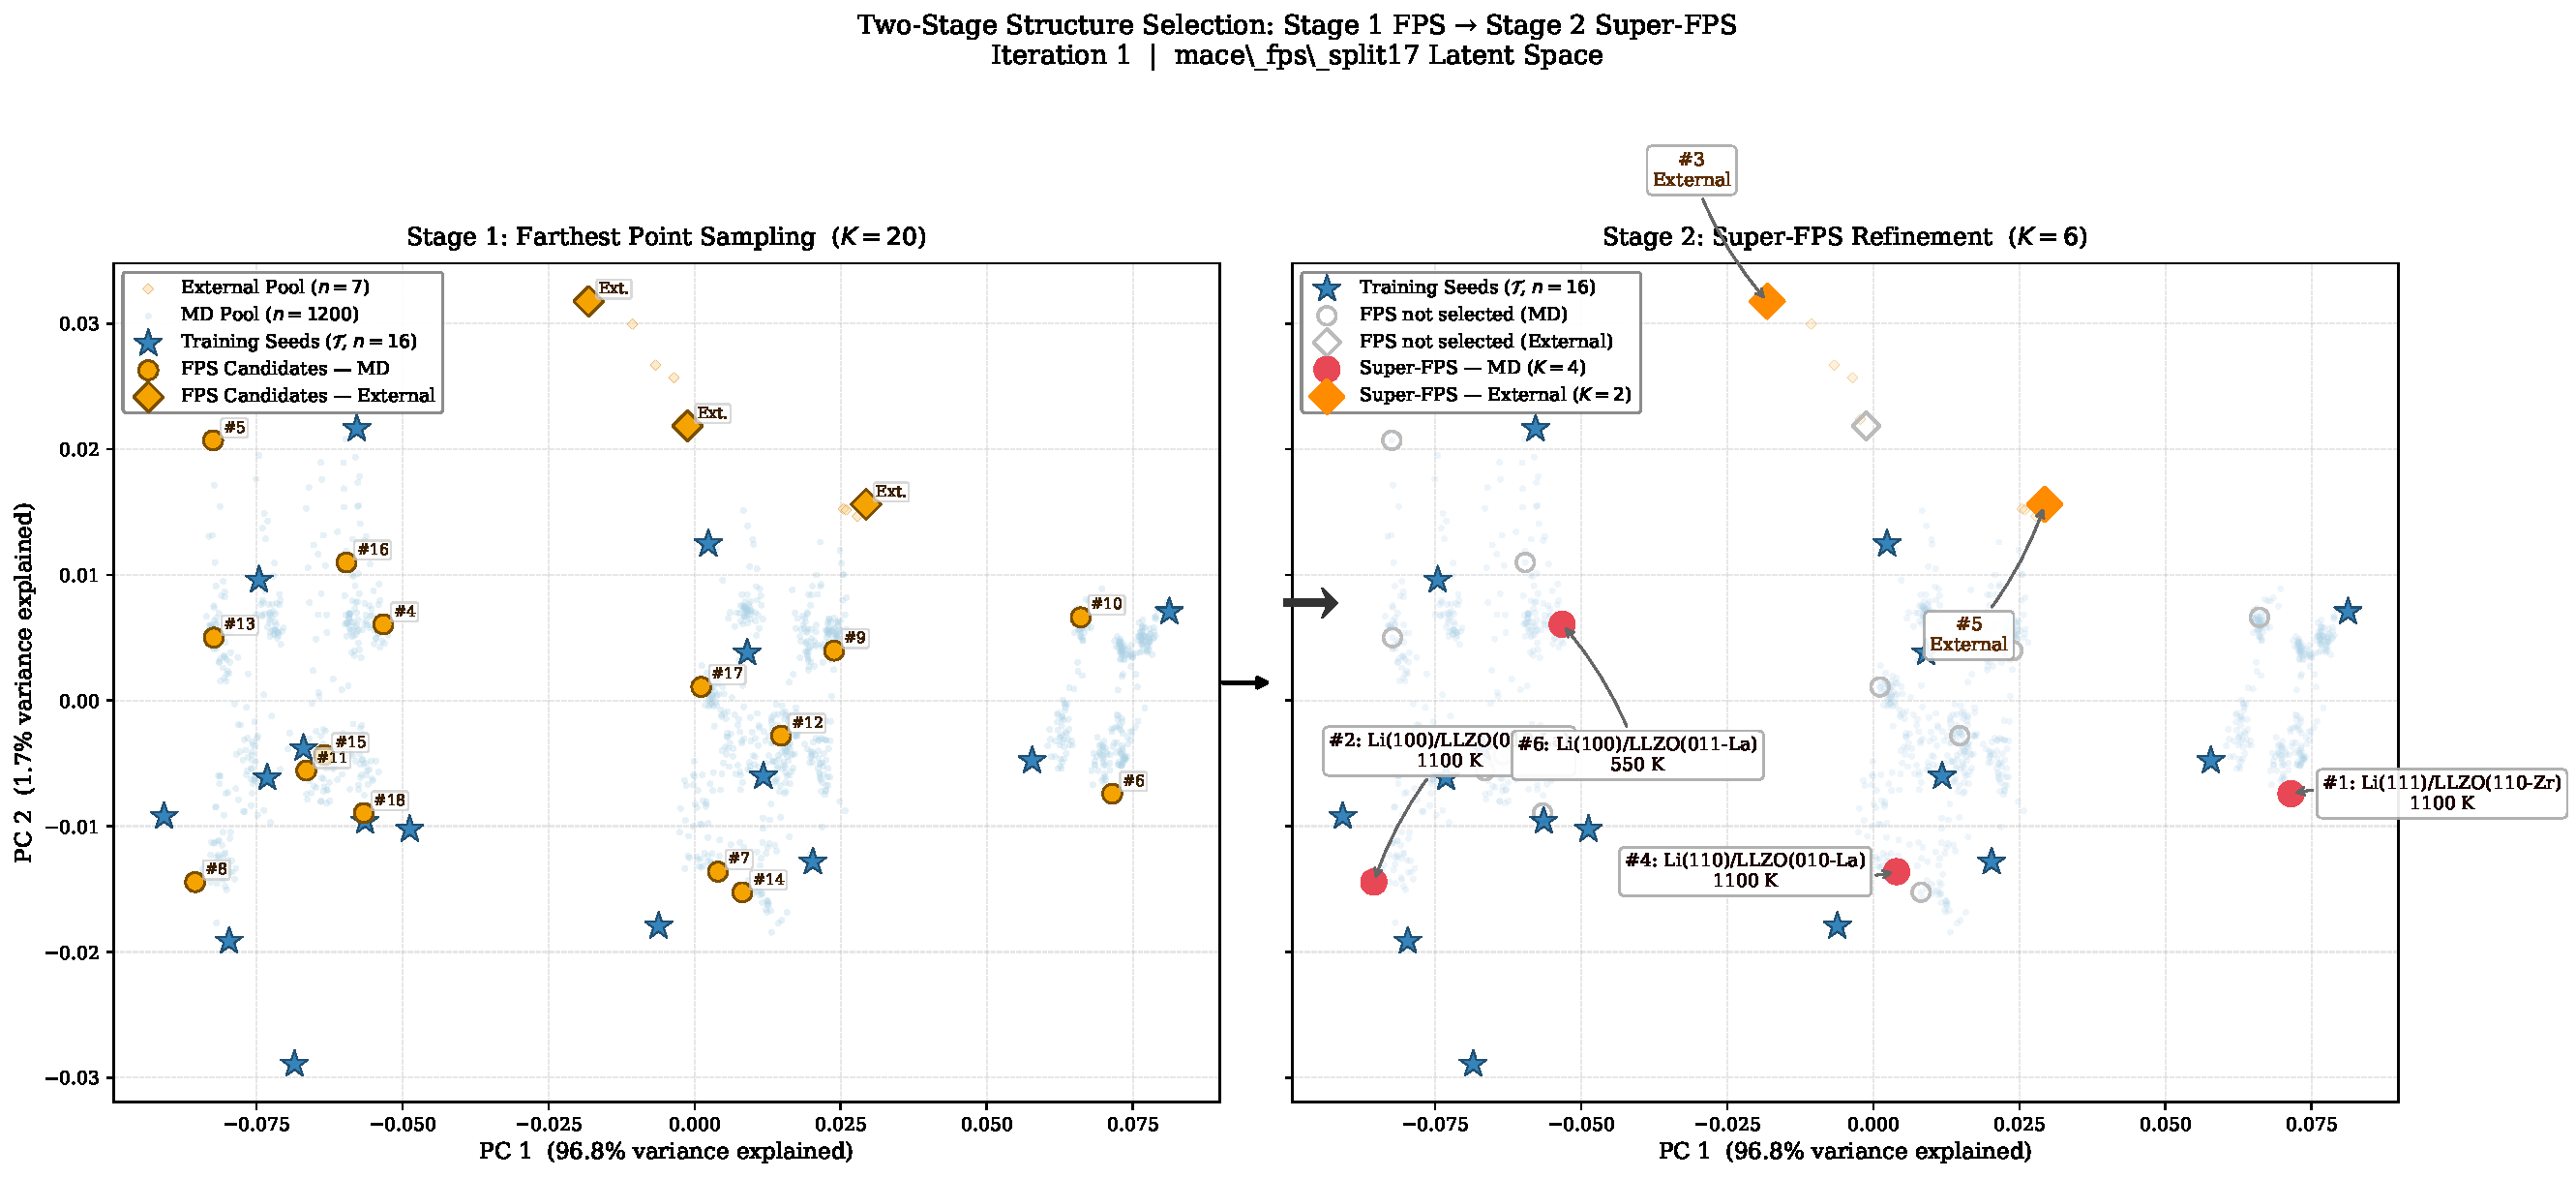
\includegraphics[width=\textwidth]{it1_split17_fps_to_superfps.pdf}\\[0.2em]
    {\footnotesize\textit{Left: Stage-1 FPS (amber circles/diamonds).
    Right: Super-FPS refinement — non-selected candidates faded;
    final 4 MD (red circles) + 2 external (orange diamonds) highlighted.
    External structures occupy an isolated cluster inaccessible to MD.}}
  \end{column}
\end{columns}
\end{frame}

%% ============================================================================
%% SLIDE 9 — DFT-FE LABELING
%% ============================================================================
\begin{frame}{Step 3: High-Fidelity DFT Labeling with DFT-FE on Frontier}
\begin{columns}[T]
  \begin{column}{0.56\textwidth}
    \textbf{Why DFT-FE for interface slabs?}
    \begin{itemize}
      \item \textbf{Native mixed BCs}: periodic in-plane, non-periodic along $\hat{z}$
        — no dipole correction or Li\,|\,LLZO\,|\,Li sandwich required
      \item Real-space FE basis: adaptive refinement near nuclei,
        coarse in vacuum — no overhead from uniform plane-wave grid
      \item Scales to $>10^5$ electrons; $\sim$20$\times$ GPU acceleration
      \item \goldtext{2023 ACM Gordon Bell Prize} (660 PFLOPS,
        620,000-electron dislocation system)
    \end{itemize}

    \vspace{0.4em}
    \textbf{Setup:} GGA-PBE, SPMS norm-conserving pseudopotentials,
    FE polynomial order 7, mesh 1.2\,\AA, SCF $5\!\times\!10^{-5}$\,Ha.\\[0.3em]
    64 nodes $\times$ 4 MI250X GPUs = 256 GPUs per job on Frontier.\\[0.3em]
    {\footnotesize BC check on 2 structures: energy diff $\sim\!10^{-6}$\,Ha;
    force diff $\sim$2.6\,meV/\AA\ $\ll$ training noise floor.}
  \end{column}
  \begin{column}{0.42\textwidth}
    \begin{block}{Dataset built by active learning}
      \centering\vspace{0.2em}
      \begin{tabular}{lcr}
        \toprule
        Iteration & +\# DFT & Atoms \\
        \midrule
        It.\ 0 & 20 & 450--1500 \\
        It.\ 1 & +6 & 450--1500 \\
        \midrule
        \textbf{Total} & \textbf{26} & --- \\
        \bottomrule
      \end{tabular}\vspace{0.2em}
    \end{block}
    \vspace{0.5em}
    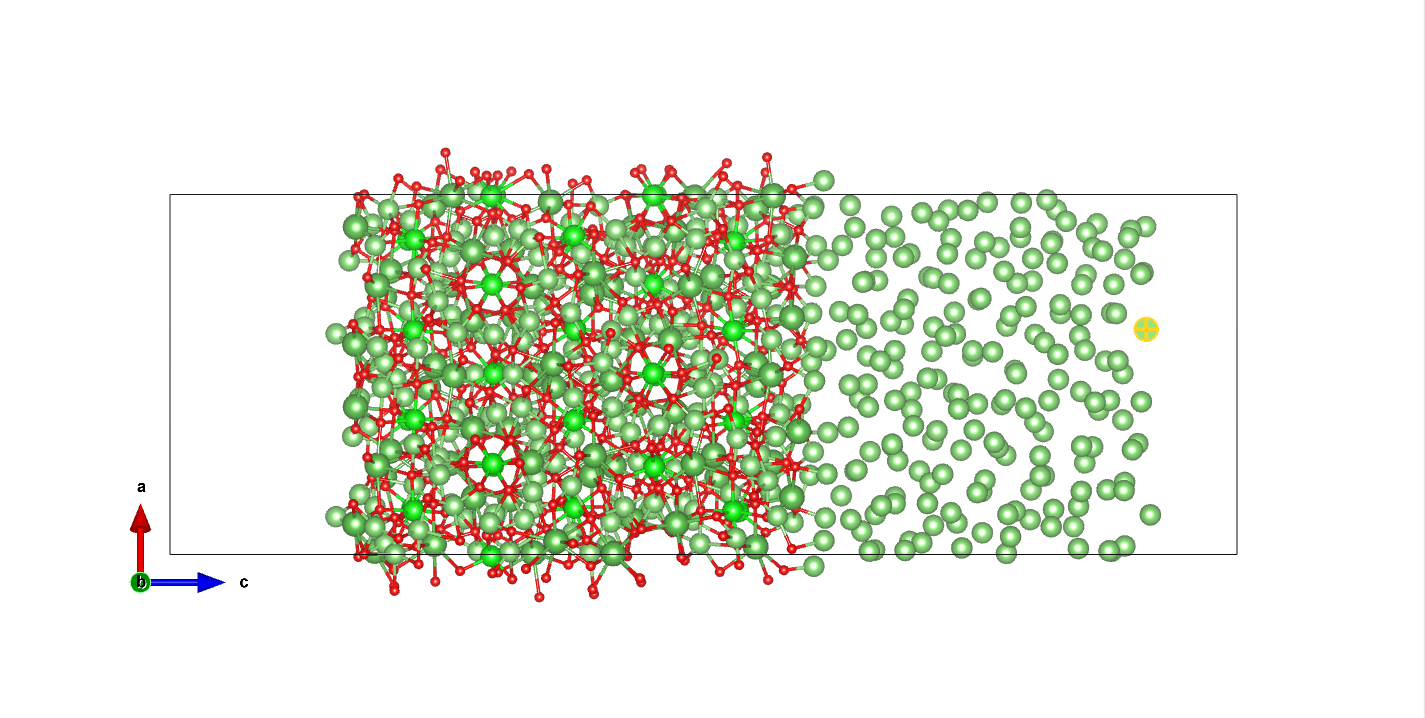
\includegraphics[width=0.48\textwidth]{non_centered.png}
    \hfill
    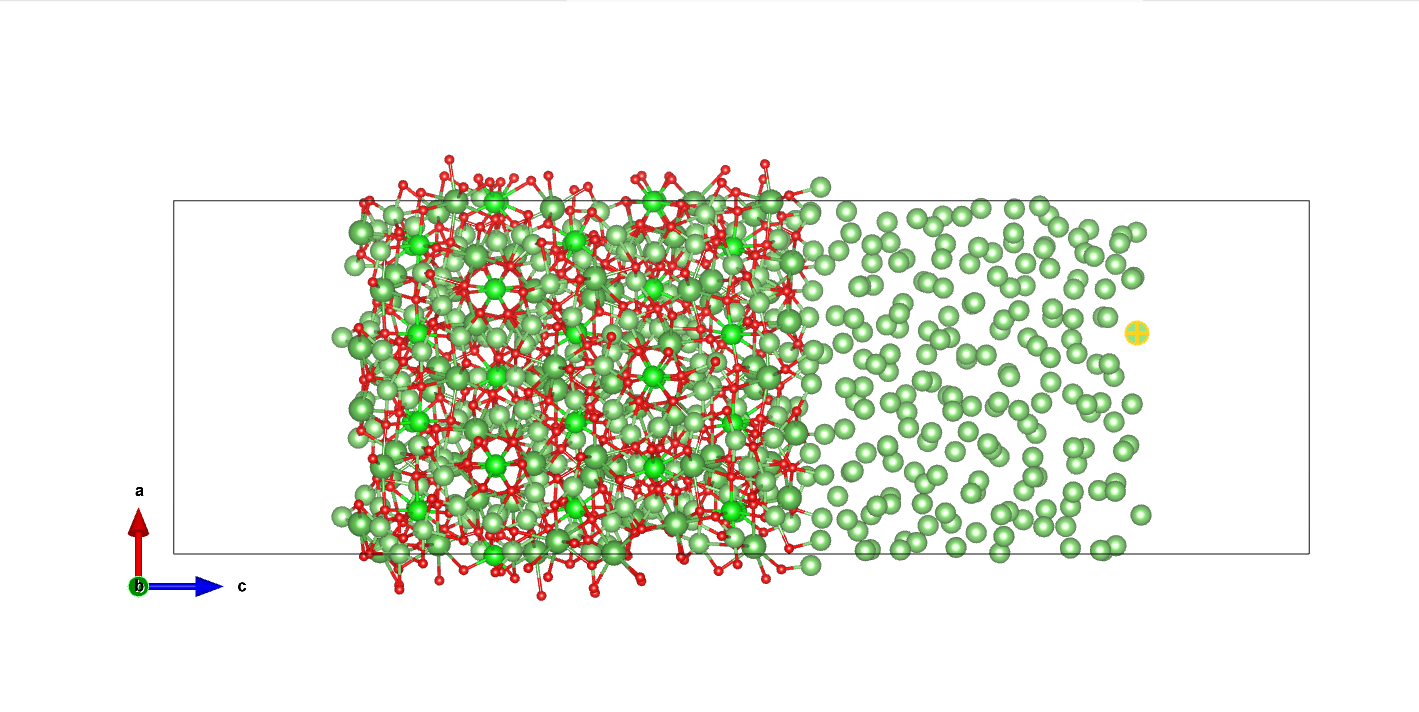
\includegraphics[width=0.48\textwidth]{centered.png}\\[0.1em]
    {\footnotesize\textit{Post-MD snapshot (left) vs.\ DFT-ready structure
    with 7.5\,\AA\ vacuum padding on each side (right).}}
  \end{column}
\end{columns}
\end{frame}

%% ============================================================================
%% SLIDE 10 — LORA FINE-TUNING
%% ============================================================================
\begin{frame}{Step 4: LoRA Fine-Tuning — Targeted Adaptation Without Forgetting}
\begin{columns}[T]
  \begin{column}{0.52\textwidth}
    \textbf{Challenge:} Full fine-tuning on 26 structures overwrites general
    MACE chemistry $\Rightarrow$ catastrophic forgetting
    \textit{[Kim et al., 2025; Springer, 2025]}.\\[0.4em]

    \textbf{Low-Rank Adaptation (LoRA):}
    \begin{equation*}
      y = \Bigl(W_0 + \tfrac{\alpha}{r} B A\Bigr) x,
      \quad B \in \mathbb{R}^{d \times r},\ A \in \mathbb{R}^{r \times d}
    \end{equation*}
    \begin{itemize}
      \item $W_0$ \textbf{frozen}; only $A,B$ trained
      \item $r\!=\!5$, $\alpha\!=\!1.0$ (hyperparameter-tuned)
      \item Trainable params: \textbf{$<$1\% of full model}
      \item Init: $B\!=\!0 \Rightarrow$ starts from pretrained behavior
      \item Equivariant LoRA applied to \texttt{o3.Linear} layers to
        preserve $O(3)$ symmetry throughout
    \end{itemize}
    \vspace{0.3em}
    \textbf{Training:} up to 300 epochs, early stopping.
    20 independent stratified splits (atom-count buckets);
    best model selected by validation loss.
  \end{column}
  \begin{column}{0.46\textwidth}
    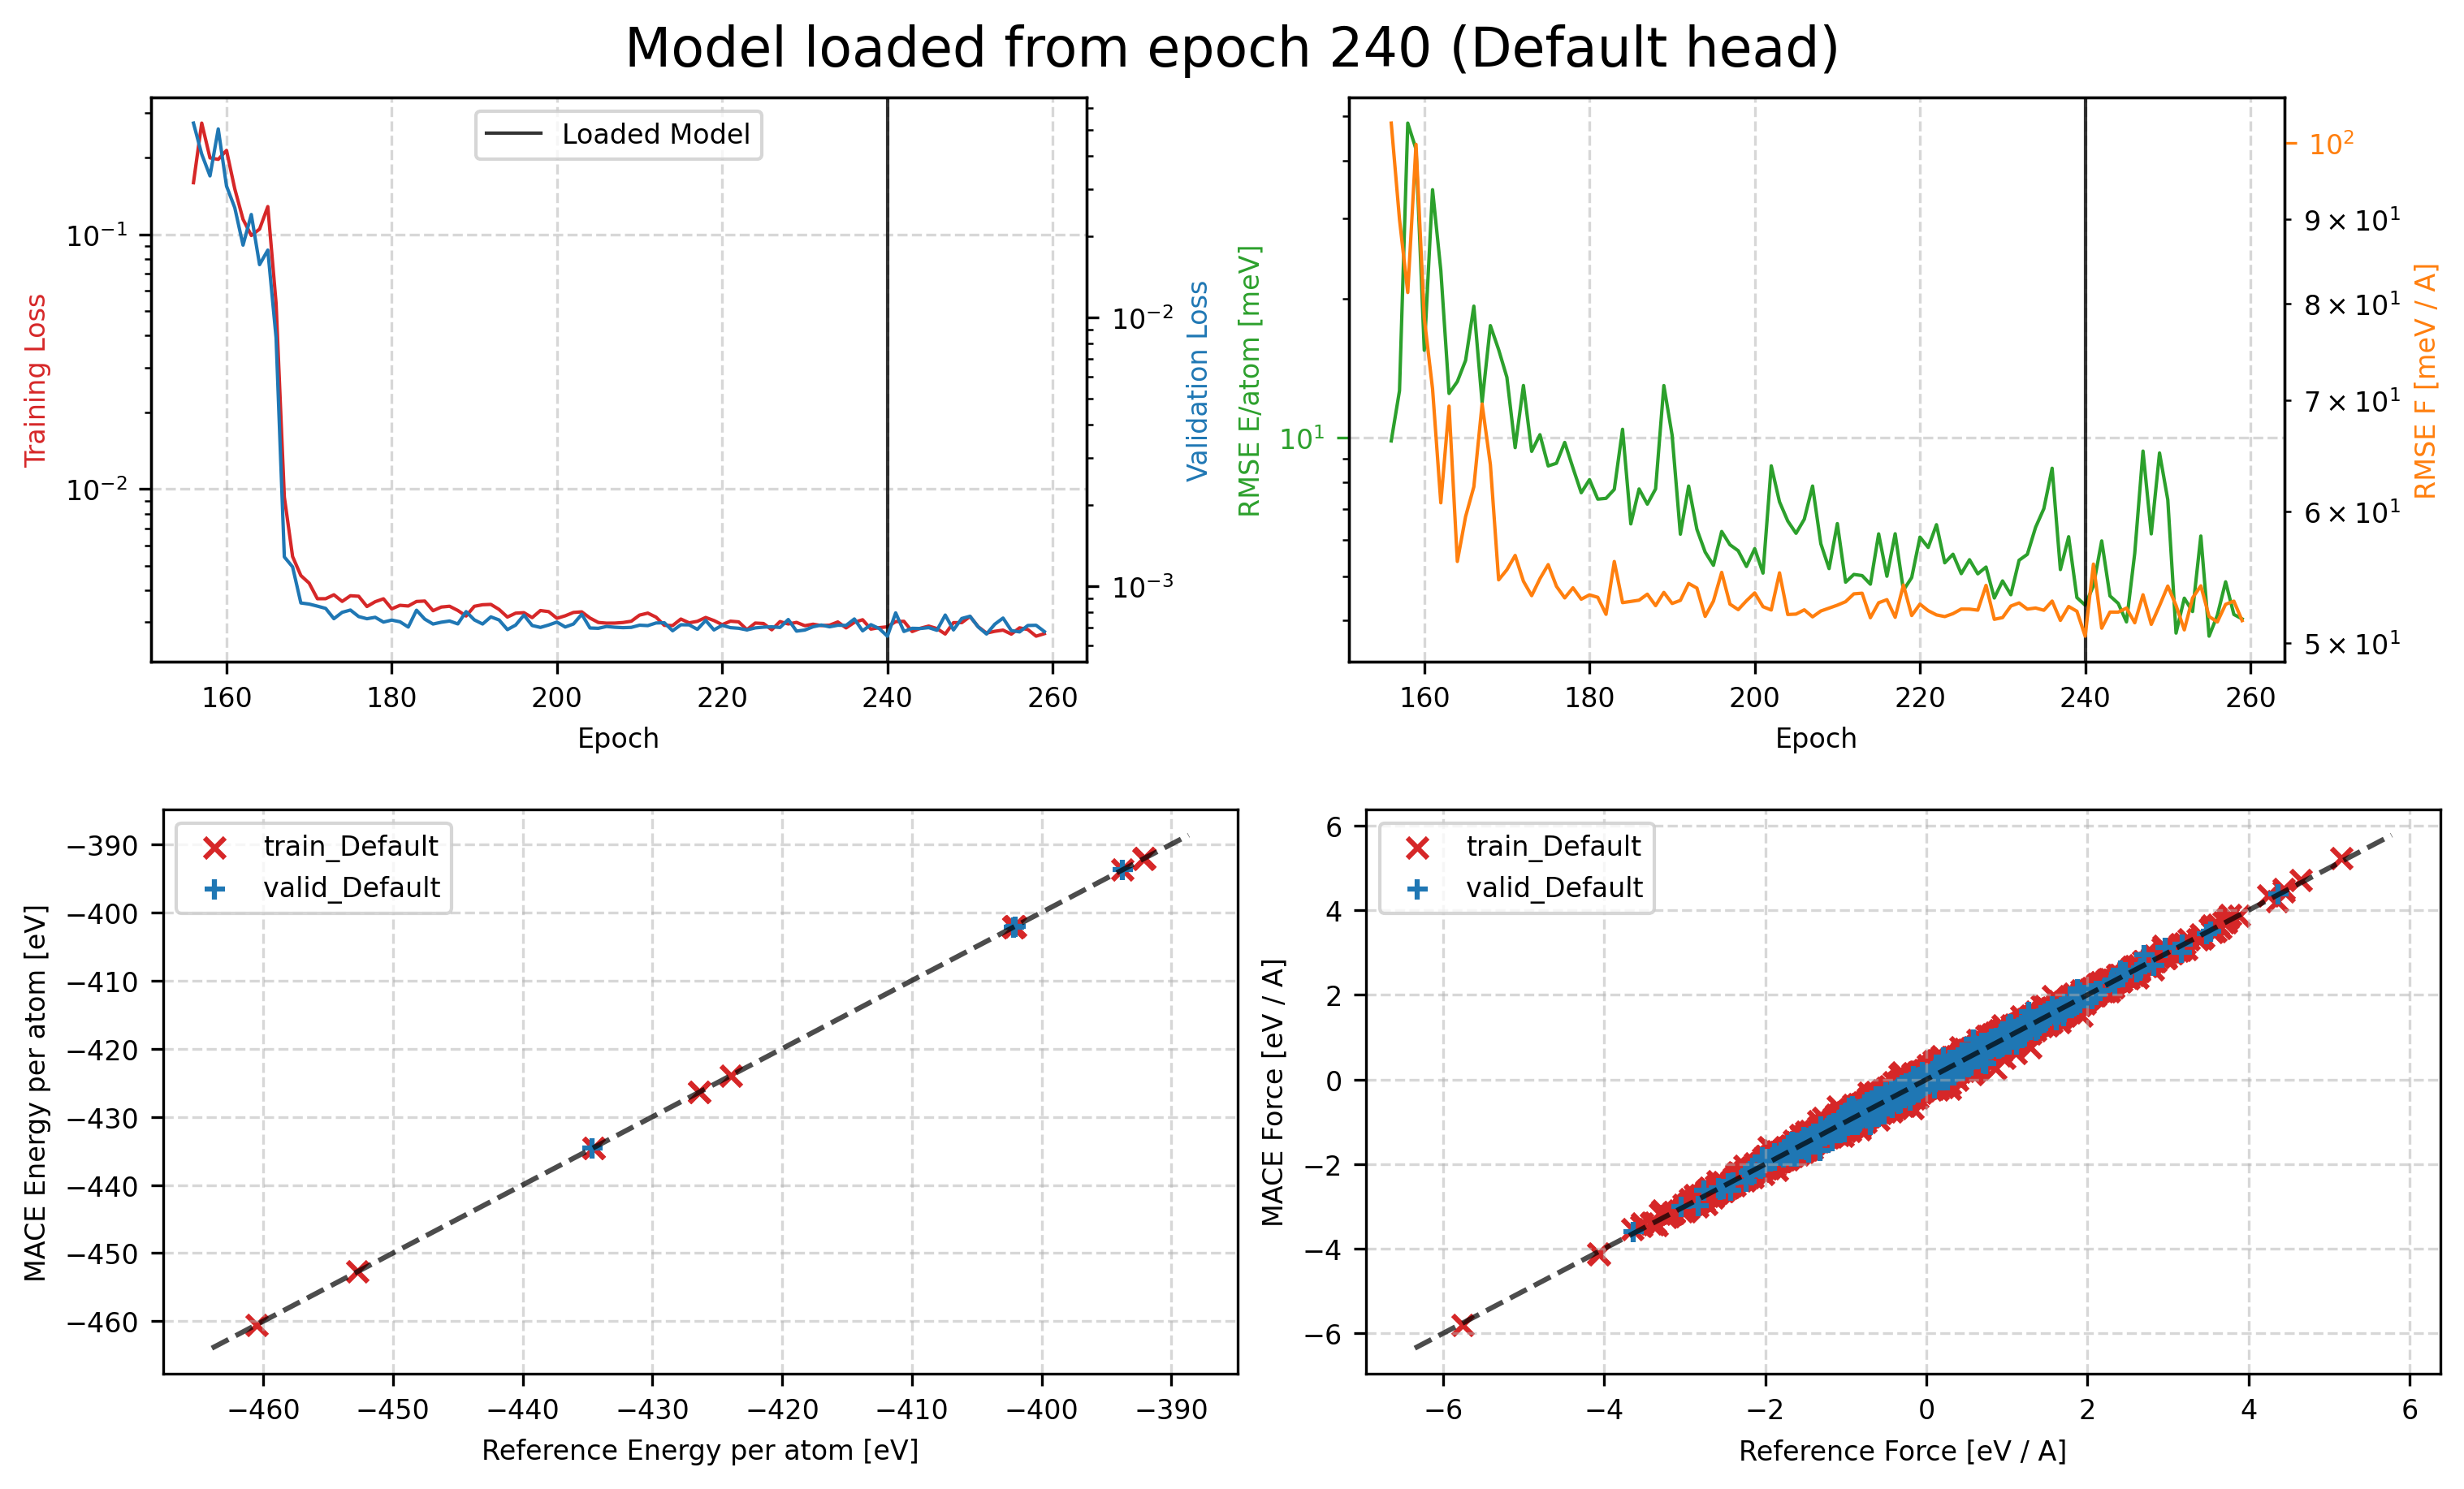
\includegraphics[width=\textwidth]{it0_finetuning_plot.png}
    {\footnotesize\textit{Iteration 0 training/validation curves.
    Energy and force RMSE converge within $\sim$180 epochs.
    No train/valid divergence throughout.}}
  \end{column}
\end{columns}
\end{frame}

%% ============================================================================
%% SLIDE 11 — BIG RESULT: ERROR REDUCTION
%% ============================================================================
\begin{frame}{Result 1: $600 \to 5$\,meV/atom in Two Iterations, 26 DFT Calls}
\begin{columns}[T]
  \begin{column}{0.5\textwidth}
    \begin{exampleblock}{Model Performance on Interface Structures}
      \centering\vspace{0.2em}
      \begin{tabular}{l@{\hspace{0.4em}}c@{\hspace{0.4em}}c@{\hspace{0.4em}}c}
        \toprule
        Model & $E$ RMSE & $F$ RMSE & Rel.\ $F$ \\
        & (meV/at.) & (meV/\AA) & (\%) \\
        \midrule
        \textbf{Universal OMAT} & \badtext{607} & \badtext{136} & --- \\
        \midrule
        \textbf{It.0 — train} & \wintext{4.6} & \wintext{51.5} & 7.97 \\
        \textbf{It.0 — valid} & \wintext{4.7} & \wintext{50.5} & 9.07 \\
        \midrule
        \textbf{It.1 — train} & \wintext{4.6} & 54.5 & 8.39 \\
        \textbf{It.1 — valid} & \wintext{3.7} & 55.4 & 9.28 \\
        \bottomrule
      \end{tabular}\vspace{0.2em}
    \end{exampleblock}

    \vspace{0.4em}
    \textbf{Key observations:}
    \begin{itemize}
      \item Train/valid errors in close agreement
        $\Rightarrow$ \wintext{no overfitting} despite 26-structure dataset
      \item Energy: $\mathbf{607 \to 4.7}$\,meV/atom
        (\goldtext{$\sim\!130\times$ improvement})
      \item Forces: $\mathbf{136 \to 50}$\,meV/\AA
        ($2.7\times$)
      \item Relative force error $\sim$9\%
        $\Rightarrow$ reliable for structural analysis and MD
    \end{itemize}
  \end{column}
  \begin{column}{0.48\textwidth}
    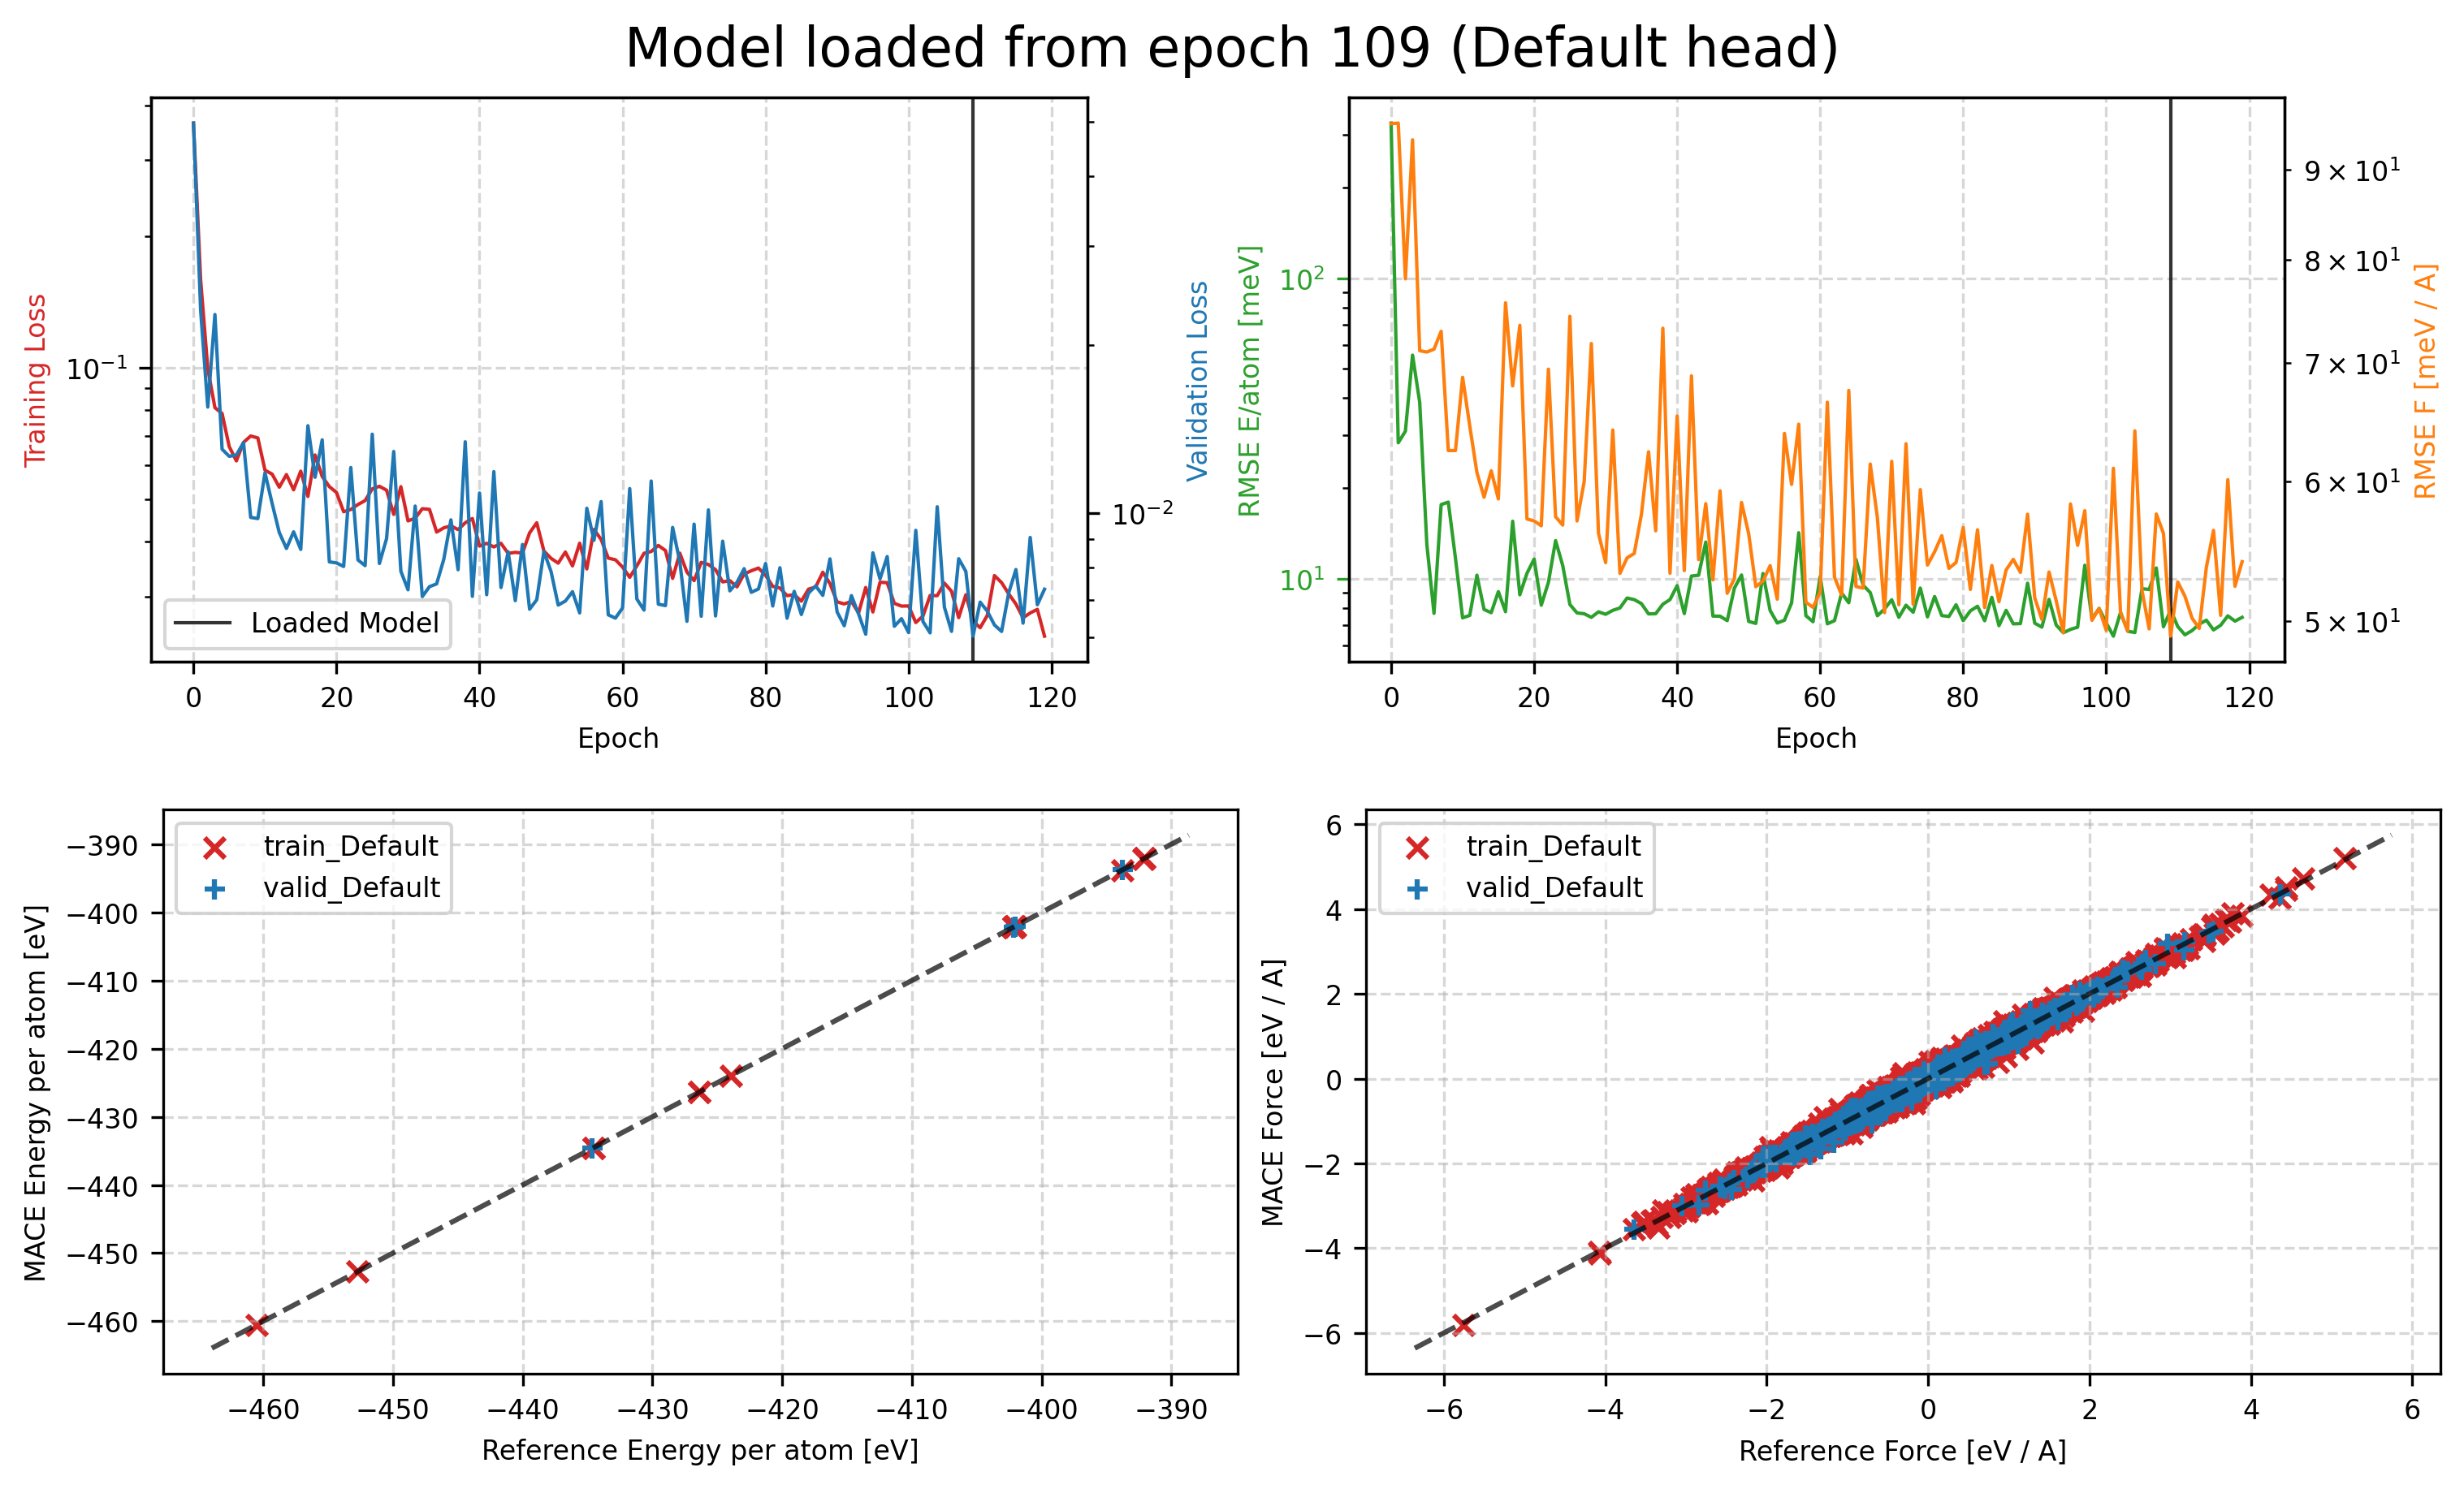
\includegraphics[width=\textwidth]{it1_ft_plt.png}
    {\footnotesize\textit{Iteration 1 training curves and parity plots.
    Smooth convergence; energy and force predictions closely track the $y\!=\!x$
    line with no systematic bias.}}
  \end{column}
\end{columns}
\end{frame}

%% ============================================================================
%% SLIDE 12 — OOD GENERALIZATION
%% ============================================================================
\begin{frame}{Result 2: Robust Out-of-Distribution Generalization}
\begin{columns}[T]
  \begin{column}{0.52\textwidth}
    \textbf{OOD test set:} 8 structures from
    \textit{Burov et al.\ (2024)} LLZO source — different Li-site occupancy,
    lattice parameters, surface termination compositions.\\
    \textit{Never seen during training.}\\[0.4em]

    {\footnotesize
    \begin{tabular}{ccccc}
      \toprule
      ID & $N$ & \multicolumn{2}{c}{CE Err (meV/at.)} & F RMSE (meV/\AA) \\
      \cmidrule(lr){3-4}
      & & It.1 & OMAT & It.1 vs OMAT \\
      \midrule
      2 & 544 & \wintext{2.6} & \badtext{16.0} & \wintext{44} vs 114 \\
      6 & 544 & \wintext{6.3} & \badtext{14.3} & \wintext{72} vs 90 \\
      1 & 776 & \wintext{1.0} & \badtext{16.6} & \wintext{96} vs 114 \\
      7 & 816 & \wintext{0.4} & \badtext{18.4} & 105 vs \badtext{202} \\
      0 & 544 & \wintext{2.6} & \badtext{15.6} & \wintext{107} vs 112 \\
      4 & 776 & \wintext{1.8} & \badtext{15.9} & 116 vs \badtext{180} \\
      5 & 544 & 5.0 & \badtext{13.3} & 137 vs \badtext{115} \\
      3 & 776 & \wintext{0.3} & \badtext{13.4} & 152 vs \badtext{127} \\
      \midrule
      \textbf{RMSE} & & \wintext{\textbf{3.21}} & \badtext{\textbf{15.5}} &
                      \wintext{\textbf{108}} vs \badtext{\textbf{136}} \\
      \bottomrule
    \end{tabular}}
  \end{column}
  \begin{column}{0.46\textwidth}
    \textbf{Universal model:} systematic \badtext{$\sim$$-15$\,meV/at.\ bias} in
    cohesive energy — consistent with PES softening even after reference alignment.\\[0.4em]

    \textbf{Fine-tuned models:} bias largely corrected; both outperform OMAT in
    almost all structures after just 2 iterations.\\[0.4em]

    \textbf{Failure cases (IDs 5, 3):} force RMSE slightly exceeds OMAT — an
    expected tension in small-data fine-tuning where energy landscape is
    learned faster than its gradients. Targeted in Iteration 3 (future work).\\[0.5em]

    \begin{block}{}
      \centering
      \textbf{26 DFT labels} $\Rightarrow$ OOD CE RMSE:\\
      \wintext{3.21} vs.\ \badtext{15.5} meV/at.\ (universal)
    \end{block}
  \end{column}
\end{columns}
\end{frame}

%% ============================================================================
%% SLIDE 13 — INTERFACE ENERGETICS
%% ============================================================================
\begin{frame}{Result 3: Interface Energetics Consistent with Prior DFT}
\begin{columns}[T]
  \begin{column}{0.52\textwidth}
    \textbf{Test:} 12 fully relaxed Li\,|\,LLZO interfaces\\
    (6$\times$ Li(001)/LLZO(001) + 6$\times$ Li(111)/LLZO(111))\\[0.4em]

    \begin{tabular}{lcc}
      \toprule
      Quantity & This work & Iwasaki et al.\ (2022) \\
      \midrule
      $\gamma_\text{int}$ (eV/\AA$^2$) & 0.118--0.338 & 0.02--0.54 \\
      $W_\text{ad}$ (eV/\AA$^2$) & $-0.22$ to $-0.04$ & $\approx -0.15$ to $+0.15$ \\
      \bottomrule
    \end{tabular}

    \vspace{0.5em}
    \textbf{Bulk cohesive energy validation:}
    \begin{tabular}{lccc}
      \toprule
      Model & Li (meV/at.) & LLZO (meV/at.) \\
      \midrule
      Universal  & 4.7 & \badtext{18.9} \\
      Iteration 0 & 4.1 & \wintext{0.25} \\
      Iteration 1 & 6.3 & \wintext{0.34} \\
      \bottomrule
    \end{tabular}

    \vspace{0.3em}
    LLZO bulk error: $18.9 \to 0.3$\,meV/at.\\
    \wintext{Critical for accurate interface formation energies.}\\[0.3em]
    {\footnotesize Consistent with Iwasaki et al.: no strong orientation preference;
    local atomic arrangement is dominant determinant.}
  \end{column}
  \begin{column}{0.46\textwidth}
    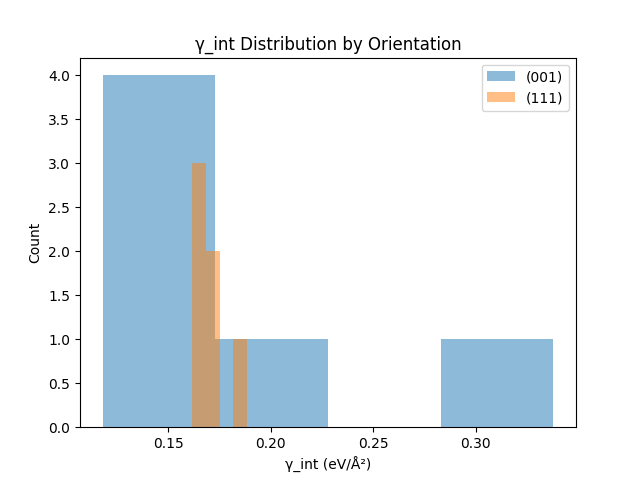
\includegraphics[width=\textwidth]{gamma_distribution_colored.png}\\[0.3em]
    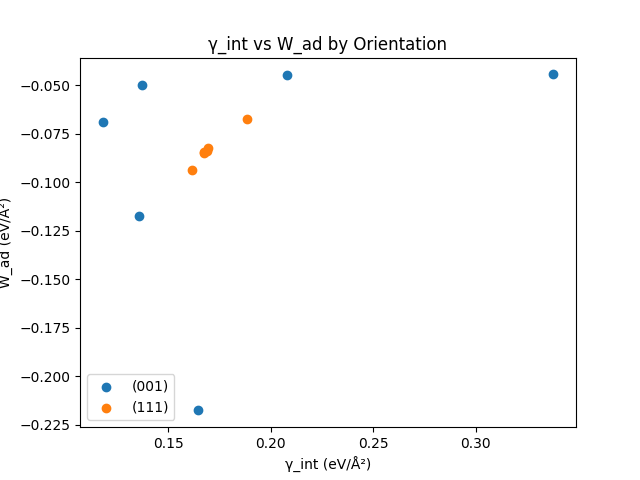
\includegraphics[width=\textwidth]{wad_vs_gamma_colored.png}\\[0.1em]
    {\footnotesize\textit{All 12 $\gamma_\text{int}$ values within Iwasaki et al.\ range.
    Weak $W_\text{ad}$--$\gamma_\text{int}$ correlation reflects distinct physical
    content of the two quantities.}}
  \end{column}
\end{columns}
\end{frame}

%% ============================================================================
%% SLIDE 14 — MD STABILITY
%% ============================================================================
\begin{frame}{Result 4: MD Stability of Li(100)--LLZO(011) at 298\,K over 200\,ps}
\begin{columns}[T]
  \begin{column}{0.38\textwidth}
    \textbf{Interface:} Li(100)/LLZO(011-La),
    vacancy-containing LLZO\\
    ($W_\text{ad} = -0.183$\,eV/\AA$^2$)\\[0.2em]
    \textbf{Conditions:} NVT Langevin, 0.5\,fs timestep,
    298\,K, 200\,ps\\[0.4em]

    \textbf{Key results:}
    \begin{itemize}
      \item \wintext{Zero Li penetration} beyond 2\,\AA\ at any timestep
      \item LLZO framework RMSD stable at $\sim$0.28\,\AA
      \item Correct mobility hierarchy:\\
        $\text{Li}_\text{metal} > \text{Li}_\text{oxide} > \text{framework}$
      \item Interface well-defined; no intermixing or structural collapse
    \end{itemize}
    \vspace{0.3em}
    \begin{alertblock}{Important caveat}
      {\footnotesize MD analysis is \textbf{qualitative}. Force errors in OOD
      regimes limit quantitative conclusions. NEB barriers + RDF comparison
      against DFT snapshots: future work.}
    \end{alertblock}
  \end{column}
  \begin{column}{0.6\textwidth}
    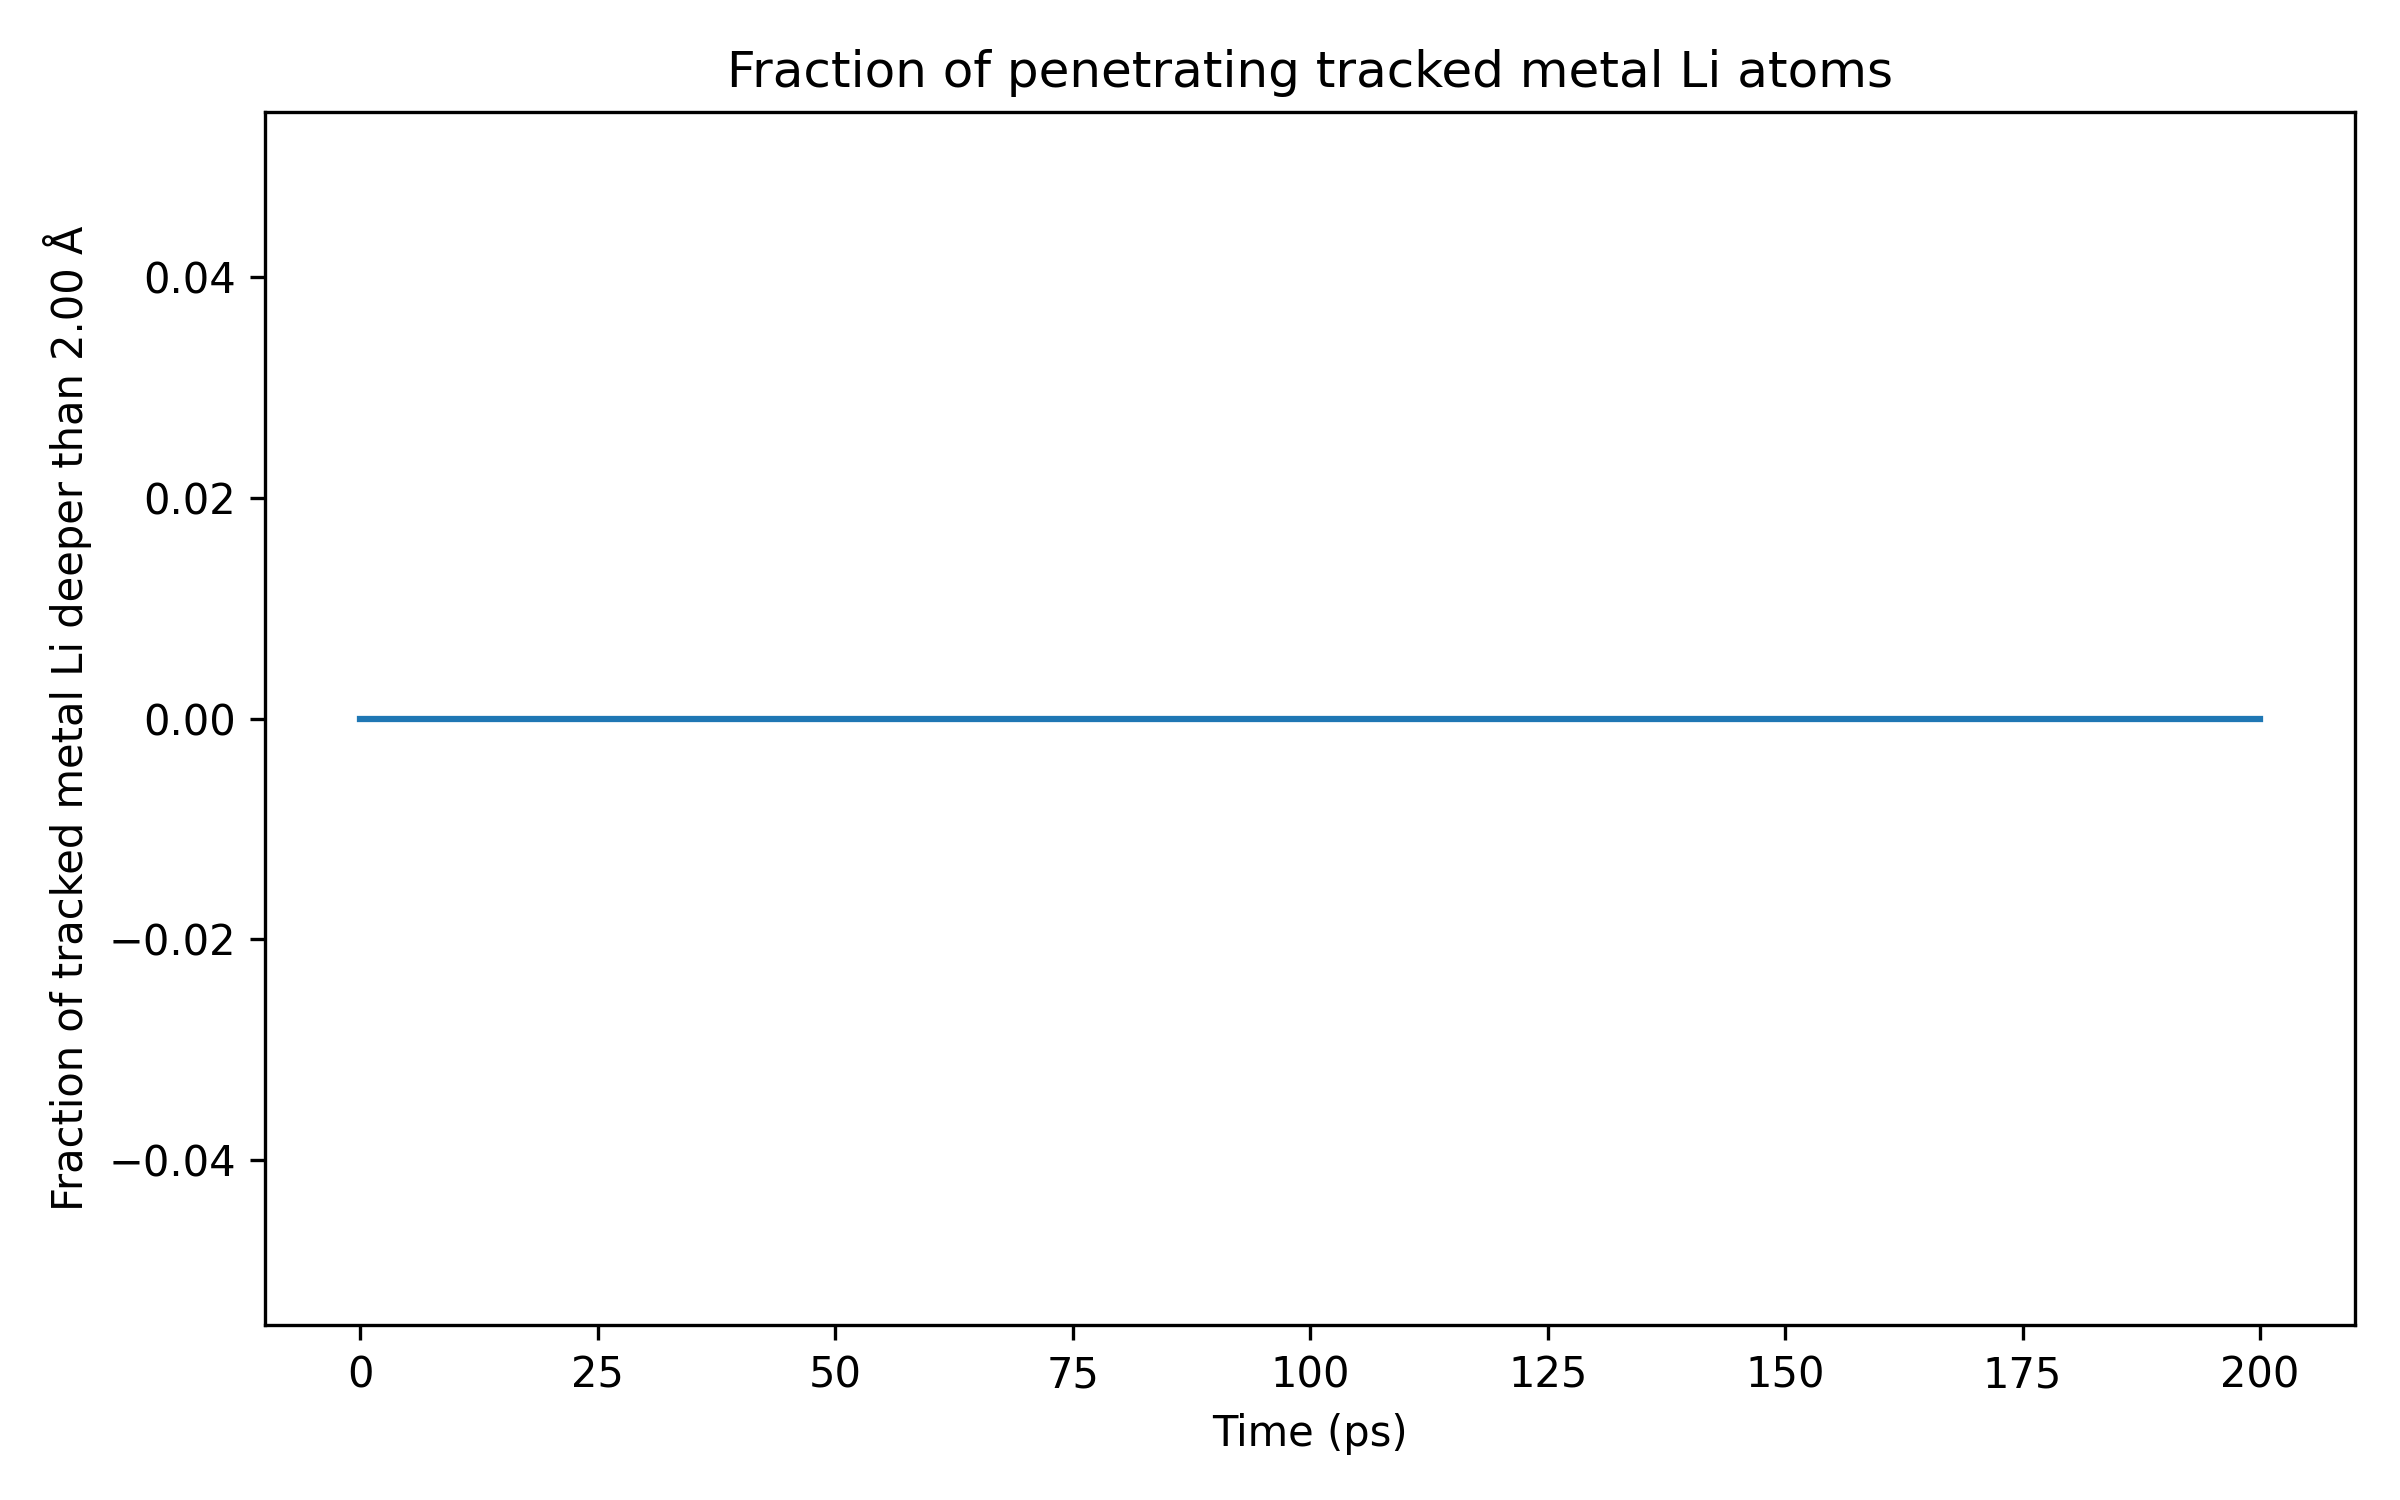
\includegraphics[width=0.49\textwidth]{li_penetration_fraction.png}
    \hfill
    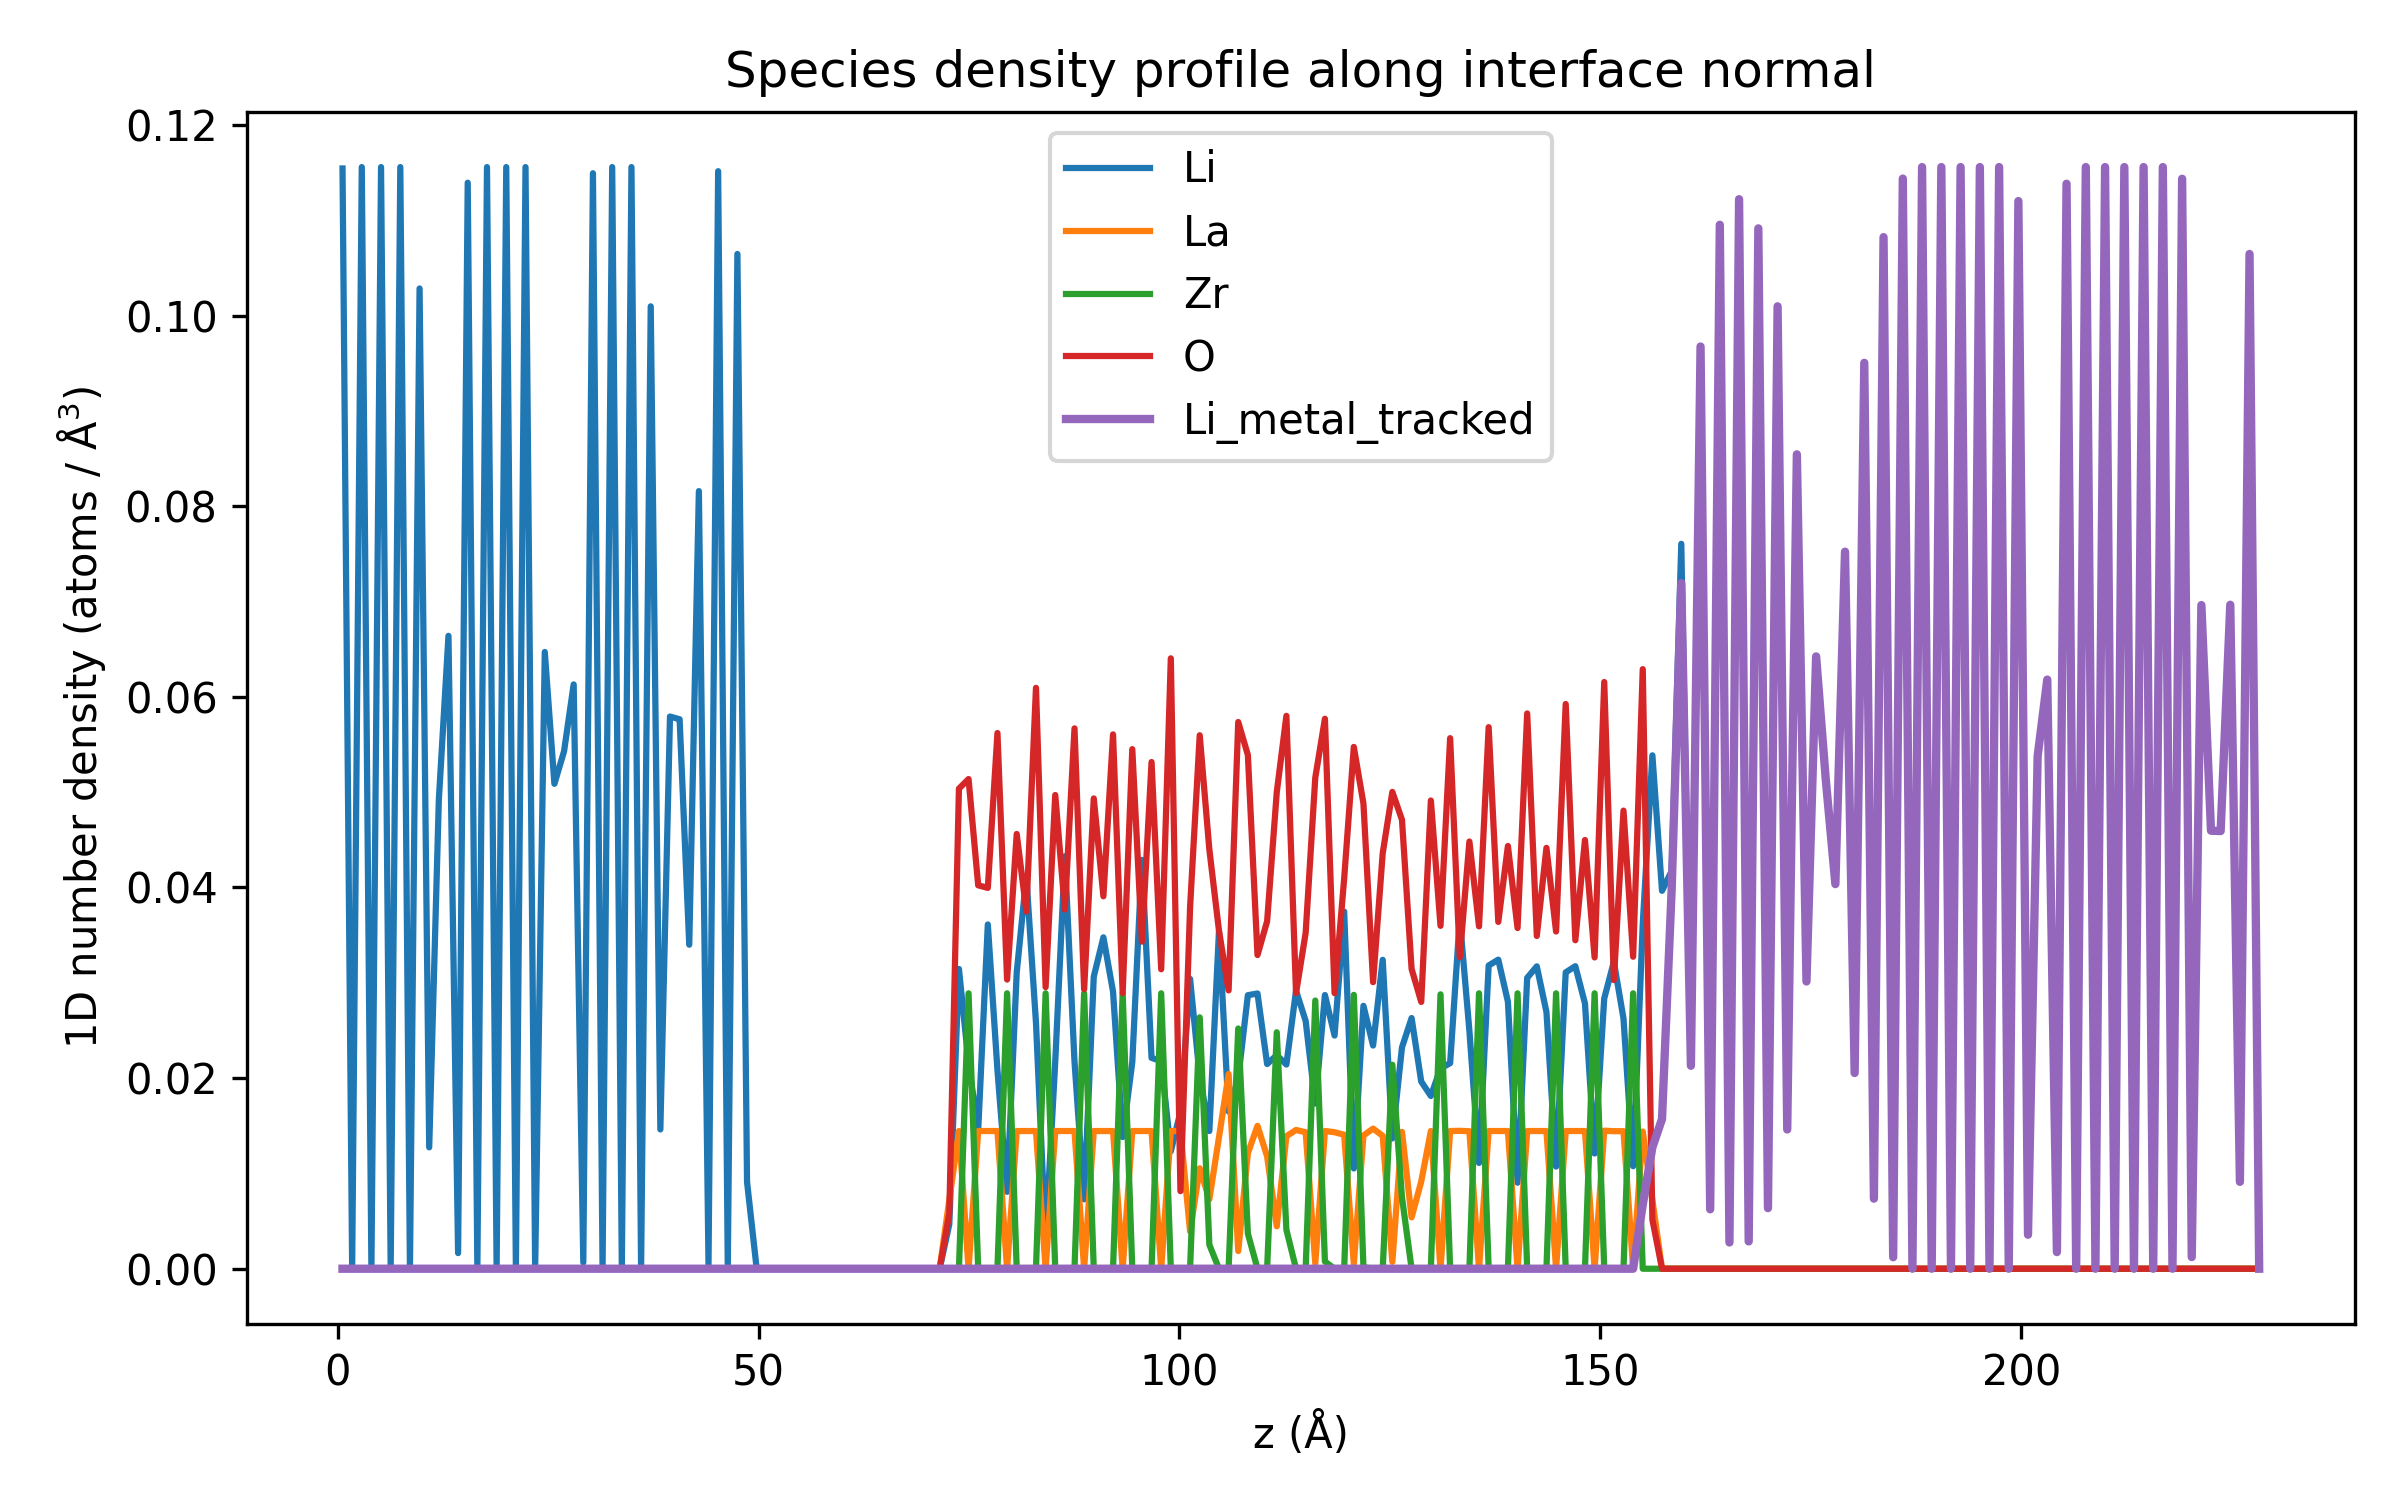
\includegraphics[width=0.49\textwidth]{z_density_profile.png}\\[0.2em]
    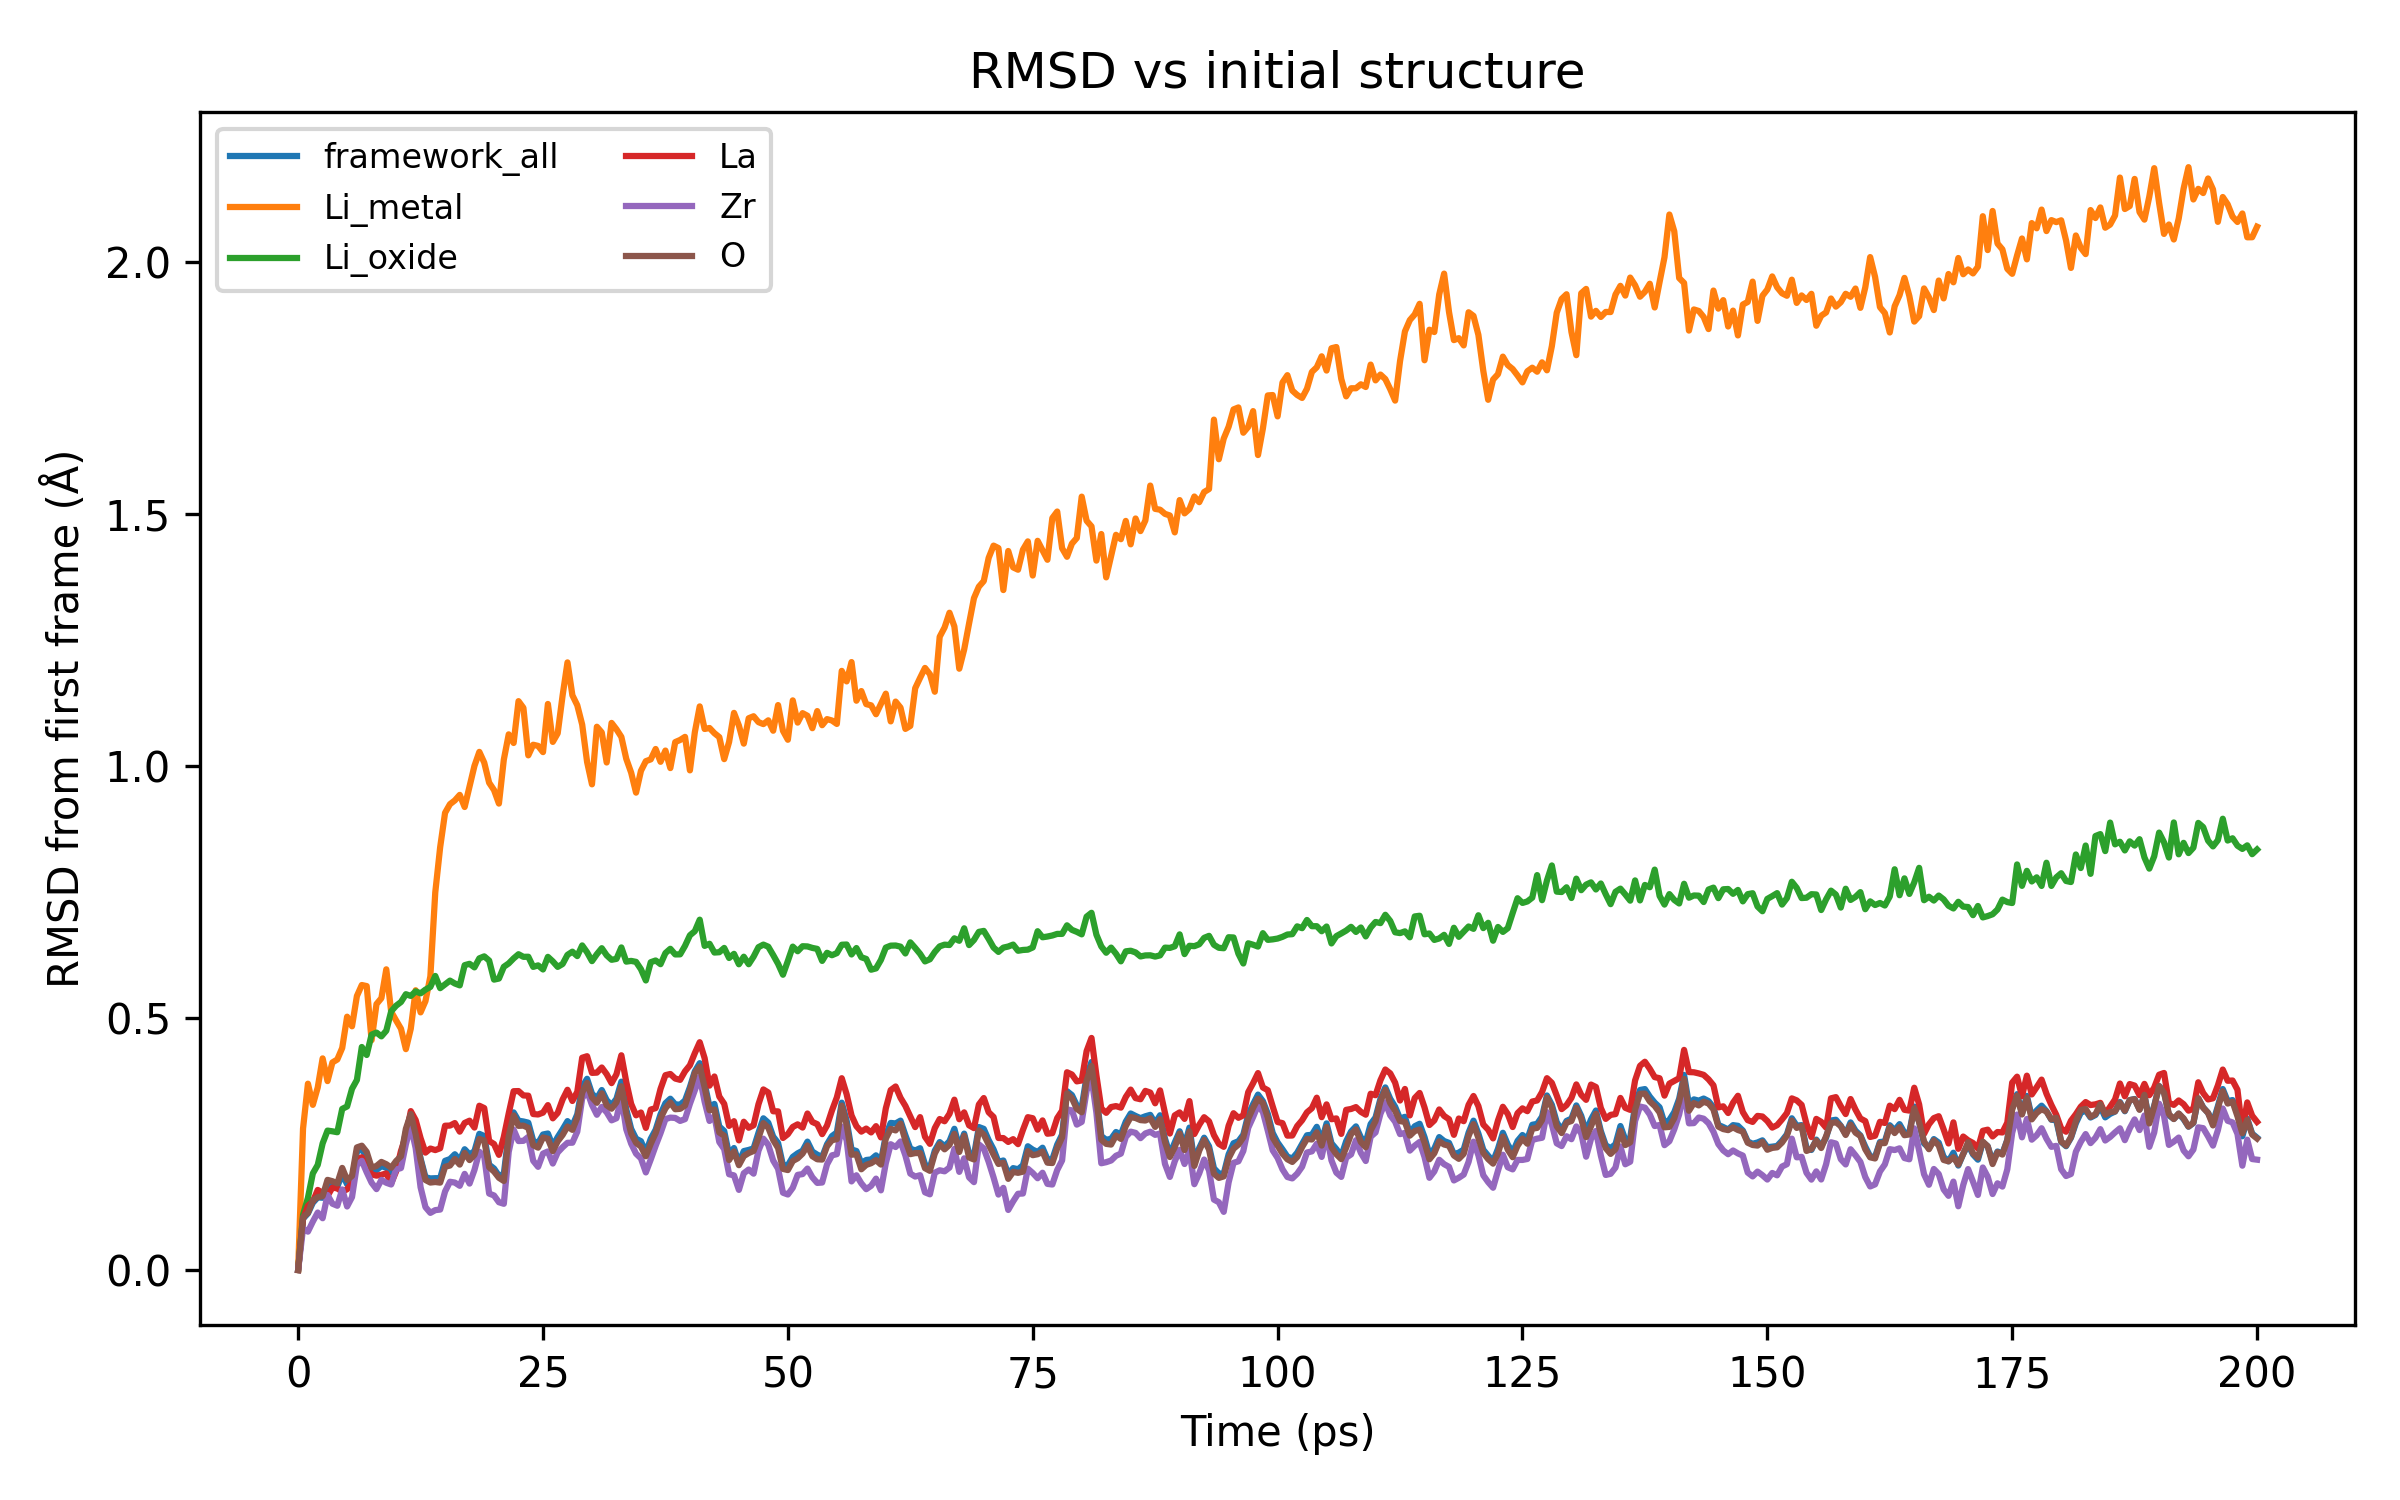
\includegraphics[width=0.49\textwidth]{rmsd_species.png}
    \hfill
    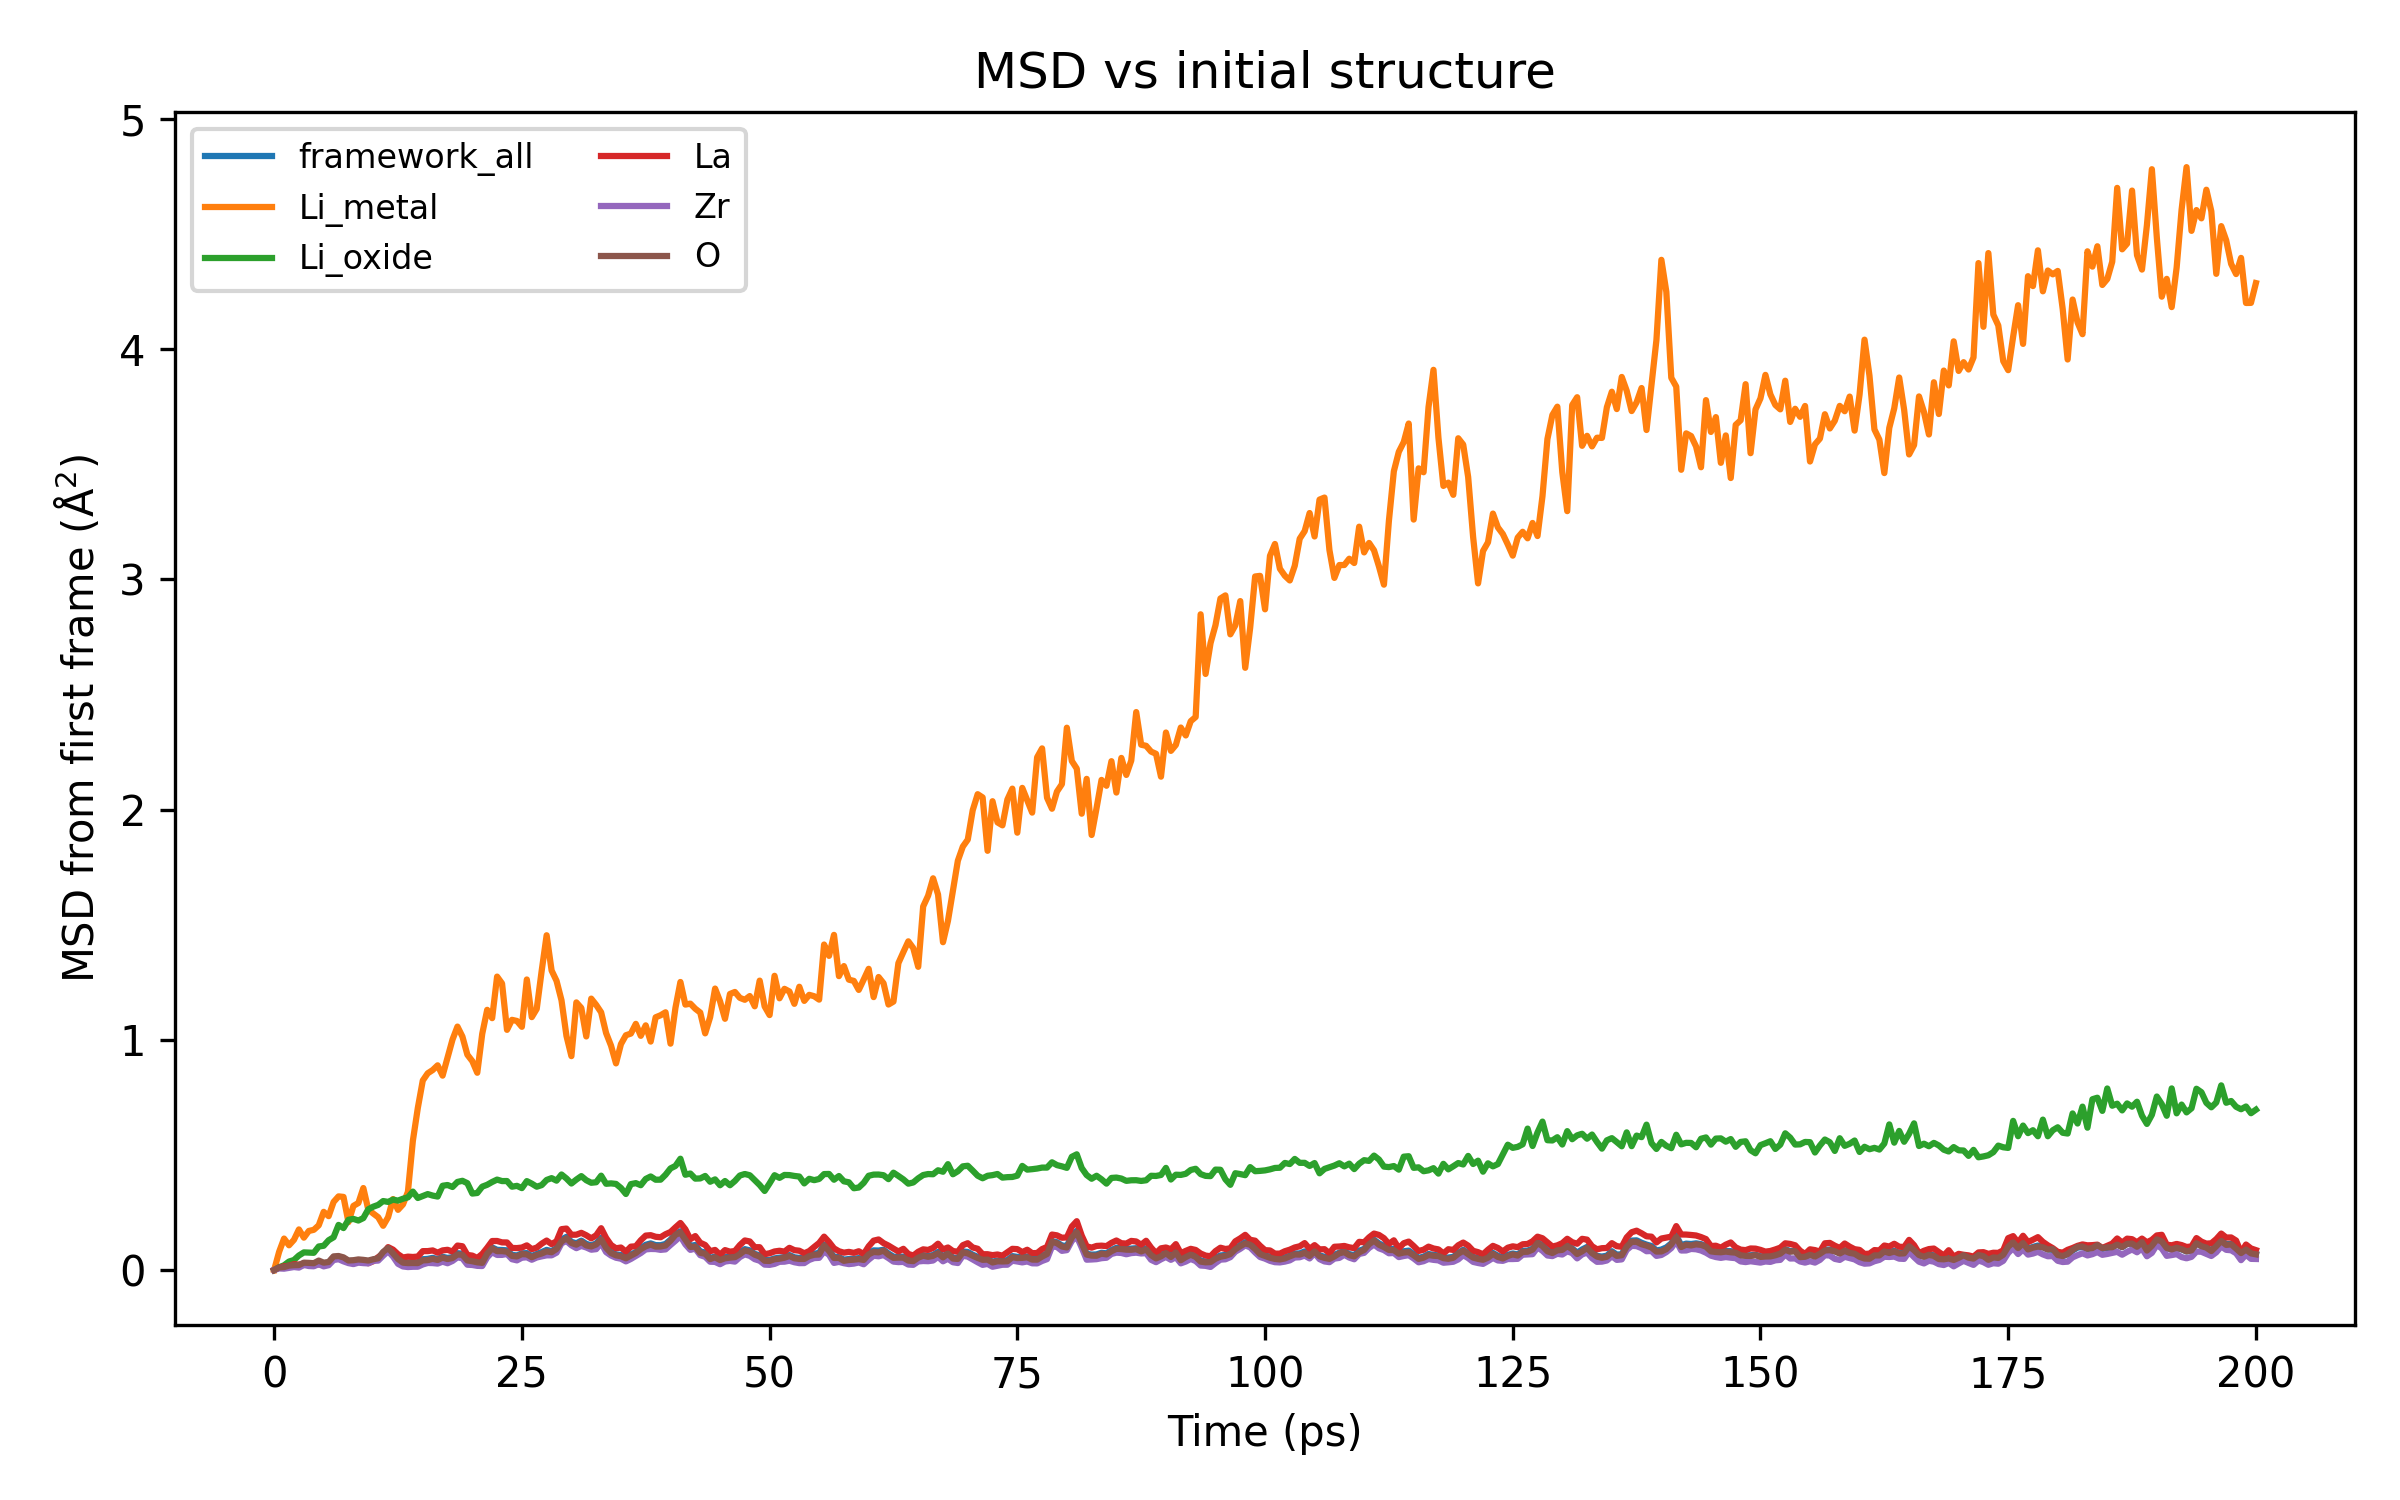
\includegraphics[width=0.49\textwidth]{msd_species.png}\\[0.15em]
    {\footnotesize\textit{Top-left: Li penetration fraction $\equiv 0$.
    Top-right: $z$-density profile — La, Zr, O confined to oxide slab.
    Bottom-left: RMSD by species (framework stable).
    Bottom-right: MSD (Li$_\text{metal}$ most mobile).}}
  \end{column}
\end{columns}
\end{frame}

%% ============================================================================
%% SLIDE 15 — CONCLUSIONS
%% ============================================================================
\begin{frame}{Summary and Future Directions}
\begin{columns}[T]
  \begin{column}{0.55\textwidth}
    \textbf{What this work establishes:}
    \begin{enumerate}
      \item \goldtext{Latent-space FPS} over MACE embeddings
        outperforms uncertainty sampling for interface MLIP training:\\
        \wintext{$\mathbf{607 \to 4.7}$\,meV/atom with 20 DFT labels}
      \item \goldtext{Super-FPS} (novel, 2-stage) enables scalable,
        non-redundant selection from large MD pools:\\
        6 structures cover 69.8\% of pool as nearest neighbors
      \item \goldtext{LoRA fine-tuning} ($r\!=\!5$) corrects PES softening
        without catastrophic forgetting
      \item \goldtext{OOD robustness:} CE RMSE $3.21$ vs.\ $15.5$\,meV/at.\
        (universal) on unseen LLZO source
      \item \goldtext{Physical validity:} energetics within Iwasaki et al.\
        DFT range; MD confirms structural stability at 298\,K
    \end{enumerate}
  \end{column}
  \begin{column}{0.43\textwidth}
    \textbf{Immediate next steps:}
    \begin{itemize}
      \item Iteration 3: tetragonal LLZO from Iwasaki et al.\ as pool members
      \item NEB Li migration barriers vs.\ DFT-NEB reference
      \item RDF/ADF comparison: MLIP-MD vs.\ DFT-labeled MD snapshots
      \item Quantitative Li diffusivity at 600--900\,K
      \item Systematic LoRA rank study with larger dataset
    \end{itemize}
    \vspace{0.5em}
    \begin{block}{General framework}
      {\small Latent FPS + Super-FPS + LoRA is
      \textbf{architecture-agnostic}
      and directly transferable to Li$|$LPS, Li$|$LIPON,
      NaSICON, and other solid-electrolyte interfaces.}
    \end{block}
  \end{column}
\end{columns}
\vspace{0.3em}
\begin{center}
  {\small\textit{Code and data available on request.}}
\end{center}
\end{frame}

%% ============================================================================
%% SLIDE 16 — ACKNOWLEDGEMENTS
%% ============================================================================
\begin{frame}{Acknowledgements}
\begin{columns}[T]
  \begin{column}{0.62\textwidth}
    \begin{itemize}
      \item \textbf{Prof.\ Phani Motamarri} — primary supervision,
        DFT-FE codebase, OLCF Frontier allocation
      \item \textbf{Prof.\ Sai Gautam Gopalakrishnan} — co-supervision,
        LLZO surface structures (Canepa et al., 2018),
        conceptual guidance on interface physics
      \item \textbf{Kartick \& Rajdeep} (MATRIX Lab) — constant
        intellectual input and support
      \item \textbf{MATRIX Lab} (Naman, Gourab, Harshit, Atharva)
      \item \textbf{Prof.\ G.\ P.\ Das}
      \item \textbf{OLCF Frontier} — DFT-FE calculations
      \item \textbf{KIAC Mahamathi cluster \& ALCF Polaris} —
        ML training and MD simulations
    \end{itemize}
  \end{column}
  \begin{column}{0.35\textwidth}
    \centering
    
\includegraphics[height=2.8cm]{iisc_logo.jpg}\\[0.6em]
    {\Large\textbf{Thank you.}}\\[0.5em]
    {\normalsize Questions?}
  \end{column}
\end{columns}
\end{frame}

\end{document}